\subsection{Thiết kế cơ sở dữ liệu}
\begin{figure}[H]
    \centering
    \includegraphics[width=0.95\textwidth]{Images/Design/DB/EERD.png}
    \caption{Sơ đồ cơ sở dữ liệu của hệ thống}
    \label{fig:database-diagram}
\end{figure}

\newlength{\colField} \setlength{\colField}{2.5cm}
\newlength{\colConst} \setlength{\colConst}{5.5cm}
\newlength{\colDesc}  \setlength{\colDesc}{7.0cm}

\subsubsection{Các thực thể chính}

% ==========================================
% 1. Bảng users
% ==========================================
\begin{longtable}{p{\colField} p{\colConst} p{\colDesc}}
    \caption{Bảng users (Bảng cha, Single Table Inheritance)} \label{tab:users} \\
    \toprule
    \textbf{Trường} & \textbf{Ràng buộc} & \textbf{Mô tả / Ghi chú} \\
    \midrule
    \endfirsthead
    
    \multicolumn{3}{c}{\tablename\ \thetable\ -- tiếp theo} \\
    \toprule
    \textbf{Trường} & \textbf{Ràng buộc} & \textbf{Mô tả / Ghi chú} \\
    \midrule
    \endhead
    
    \bottomrule
    \endlastfoot

    id & PK, NOT NULL & Khóa chính (UUID) \\
    full\_name & NOT NULL & Họ và tên đầy đủ \\
    email & UNIQUE, NOT NULL & Email đăng nhập hệ thống \\
    phone & UNIQUE, NOT NULL & Số điện thoại liên lạc \\
    avatar\_url & NULL & Đường dẫn ảnh đại diện \\
    password\_hash & NOT NULL & Mật khẩu đã mã hóa \\
    status & NOT NULL, default 'ACTIVE' & ENUM: ACTIVE, INACTIVE, SUSPENDED, BANNED \\
    role & NOT NULL & ENUM: RENTER, OWNER, ADMIN \\
    trust\_score & NOT NULL, default 50 & Điểm uy tín (thang 0--100) \\
    trust\_factors & NULL & JSON chi tiết các yếu tố tính điểm \\
    trust\_last\_calculated & NULL & Thời điểm tính điểm gần nhất \\
    created\_at & NOT NULL, default NOW & Thời gian tạo tài khoản \\
    updated\_at & NOT NULL, default NOW & Thời gian cập nhật lần cuối \\
\end{longtable}

\vspace{0.5cm}

% ==========================================
% 2. Bảng renters
% ==========================================
\begin{longtable}{p{\colField} p{\colConst} p{\colDesc}}
    \caption{Bảng renters (Thuộc tính riêng người thuê)} \label{tab:renters} \\
    \toprule
    \textbf{Trường} & \textbf{Ràng buộc} & \textbf{Mô tả / Ghi chú} \\
    \midrule
    \endfirsthead
    \bottomrule
    \endlastfoot

    user\_id & PK, FK $\to$ users.id, ON DELETE CASCADE & Khóa chính đồng thời là khóa ngoại \\
    address & NULL & Địa chỉ thường trú \\
    license\_number & UNIQUE, NOT NULL & Số giấy phép lái xe \\
    verification\_status & NOT NULL, default 'PENDING' & ENUM: PENDING, VERIFIED, REJECTED \\
\end{longtable}

\vspace{0.5cm}

% ==========================================
% 3. Bảng owners
% ==========================================
\begin{longtable}{p{\colField} p{\colConst} p{\colDesc}}
    \caption{Bảng owners (Thuộc tính riêng chủ xe)} \label{tab:owners} \\
    \toprule
    \textbf{Trường} & \textbf{Ràng buộc} & \textbf{Mô tả / Ghi chú} \\
    \midrule
    \endfirsthead
    \bottomrule
    \endlastfoot

    user\_id & PK, FK $\to$ users.id, ON DELETE CASCADE & Khóa chính đồng thời là khóa ngoại \\
    bank\_account & NOT NULL (encrypted) & Số tài khoản ngân hàng (nhận tiền) \\
    id\_card\_number & NOT NULL (encrypted) & Số CMND/CCCD \\
    id\_card\_front\_url & NULL & Link ảnh mặt trước CMND/CCCD \\
    id\_card\_back\_url & NULL & Link ảnh mặt sau CMND/CCCD \\
\end{longtable}

\vspace{0.5cm}

% ==========================================
% 4. Bảng admins
% ==========================================
\begin{longtable}{p{\colField} p{\colConst} p{\colDesc}}
    \caption{Bảng admins (Thuộc tính quản trị viên)} \label{tab:admins} \\
    \toprule
    \textbf{Trường} & \textbf{Ràng buộc} & \textbf{Mô tả / Ghi chú} \\
    \midrule
    \endfirsthead
    \bottomrule
    \endlastfoot

    user\_id & PK, FK $\to$ users.id, ON DELETE CASCADE & Khóa chính đồng thời là khóa ngoại \\
    permissions & NOT NULL & Danh sách quyền hạn (mảng JSON) \\
    department & NULL & Tên bộ phận quản lý \\
\end{longtable}

\vspace{0.5cm}

% ==========================================
% 5. Bảng vehicles
% ==========================================
\begin{longtable}{p{\colField} p{\colConst} p{\colDesc}}
    \caption{Bảng vehicles (Thông tin xe)} \label{tab:vehicles} \\
    \toprule
    \textbf{Trường} & \textbf{Ràng buộc} & \textbf{Mô tả / Ghi chú} \\
    \midrule
    \endfirsthead
    \multicolumn{3}{c}{\tablename\ \thetable\ -- tiếp theo} \\
    \toprule
    \textbf{Trường} & \textbf{Ràng buộc} & \textbf{Mô tả / Ghi chú} \\
    \midrule
    \endhead
    \bottomrule
    \endlastfoot

    id & PK & Khóa chính (UUID) \\
    owner\_id & FK $\to$ users.id (role=OWNER), NOT NULL & Liên kết tới chủ sở hữu \\
    license\_plate & UNIQUE, NOT NULL & Biển số xe \\
    model & NOT NULL & Tên mẫu xe (Model) \\
    type & NOT NULL & ENUM: STANDARD, PREMIUM, HEAVY\_DUTY \\
    status & NOT NULL & ENUM: AVAILABLE, RENTED, MAINTENANCE, INACTIVE... \\
    battery\_level & NOT NULL, range 0--100 & Phần trăm pin hiện tại \\
    price\_per\_hour & NOT NULL & Đơn giá thuê theo giờ \\
    latitude & NOT NULL & Vĩ độ vị trí hiện tại \\
    longitude & NOT NULL & Kinh độ vị trí hiện tại \\
    total\_rating & default 0 & Điểm đánh giá trung bình \\
    total\_trips & default 0 & Tổng số chuyến đi đã thực hiện \\
    image\_urls & NULL & Mảng JSON chứa link ảnh xe \\
    created\_at & NOT NULL, default NOW & Thời gian đăng ký xe \\
\end{longtable}

\vspace{0.5cm}

% ==========================================
% 6. Bảng bookings
% ==========================================
\begin{longtable}{p{\colField} p{\colConst} p{\colDesc}}
    \caption{Bảng bookings (Đơn đặt xe)} \label{tab:bookings} \\
    \toprule
    \textbf{Trường} & \textbf{Ràng buộc} & \textbf{Mô tả / Ghi chú} \\
    \midrule
    \endfirsthead
    \multicolumn{3}{c}{\tablename\ \thetable\ -- tiếp theo} \\
    \toprule
    \textbf{Trường} & \textbf{Ràng buộc} & \textbf{Mô tả / Ghi chú} \\
    \midrule
    \endhead
    \bottomrule
    \endlastfoot

    id & PK & Khóa chính (UUID) \\
    renter\_id & FK $\to$ users.id (role=RENTER), NOT NULL & Người thực hiện thuê \\
    vehicle\_id & FK $\to$ vehicles.id, NOT NULL & Xe được chọn thuê \\
    start\_time & NOT NULL & Thời gian bắt đầu thuê \\
    end\_time & NOT NULL & Thời gian kết thúc dự kiến \\
    actual\_end\_time & NULL & Thời gian trả xe thực tế \\
    status & NOT NULL & ENUM: PENDING, APPROVED, ON\_TRIP, COMPLETED... \\
    total\_cost & NOT NULL & Tổng chi phí chuyến đi \\
    deposit & NOT NULL & Số tiền đặt cọc giữ xe \\
    start\_latitude & NOT NULL & Vĩ độ điểm nhận xe \\
    start\_longitude & NOT NULL & Kinh độ điểm nhận xe \\
    end\_latitude & NULL & Vĩ độ điểm trả xe \\
    end\_longitude & NULL & Kinh độ điểm trả xe \\
    created\_at & NOT NULL, default NOW & Thời gian tạo đơn \\
    updated\_at & NOT NULL, default NOW & Thời gian cập nhật trạng thái \\
\end{longtable}

\vspace{0.5cm}

% ==========================================
% 7. Bảng payments
% ==========================================
\begin{longtable}{p{\colField} p{\colConst} p{\colDesc}}
    \caption{Bảng payments (Giao dịch thanh toán)} \label{tab:payments} \\
    \toprule
    \textbf{Trường} & \textbf{Ràng buộc} & \textbf{Mô tả / Ghi chú} \\
    \midrule
    \endfirsthead
    \bottomrule
    \endlastfoot

    id & PK & Khóa chính (UUID) \\
    booking\_id & FK $\to$ bookings.id, NOT NULL & Liên kết đơn hàng \\
    transaction\_id & UNIQUE & Mã tham chiếu từ cổng thanh toán \\
    amount & NOT NULL & Số tiền giao dịch \\
    method & NOT NULL & ENUM: CARD, E\_WALLET, BANK\_TRANSFER \\
    status & NOT NULL & ENUM: PENDING, COMPLETED, FAILED, REFUNDED \\
    processed\_at & NULL & Thời điểm xử lý xong \\
    failure\_reason & NULL & Lý do thất bại (nếu có) \\
\end{longtable}

\vspace{0.5cm}

% ==========================================
% 8. Bảng reviews
% ==========================================
\begin{longtable}{p{\colField} p{\colConst} p{\colDesc}}
    \caption{Bảng reviews (Đánh giá chuyến đi)} \label{tab:reviews} \\
    \toprule
    \textbf{Trường} & \textbf{Ràng buộc} & \textbf{Mô tả / Ghi chú} \\
    \midrule
    \endfirsthead
    \bottomrule
    \endlastfoot

    id & PK & Khóa chính (UUID) \\
    booking\_id & FK $\to$ bookings.id, UNIQUE, NOT NULL & Mỗi chuyến đi chỉ có 1 đánh giá \\
    rating & NOT NULL, range 1--5 & Số sao đánh giá \\
    comment & NULL & Nội dung nhận xét chi tiết \\
    is\_pending & NOT NULL, default TRUE & Cờ báo trạng thái chờ duyệt \\
    created\_at & NOT NULL, default NOW & Thời gian viết đánh giá \\
\end{longtable}

\vspace{0.5cm}

% ==========================================
% 9. Bảng issues
% ==========================================
\begin{longtable}{p{\colField} p{\colConst} p{\colDesc}}
    \caption{Bảng issues (Báo cáo sự cố)} \label{tab:issues} \\
    \toprule
    \textbf{Trường} & \textbf{Ràng buộc} & \textbf{Mô tả / Ghi chú} \\
    \midrule
    \endfirsthead
    \bottomrule
    \endlastfoot

    id & PK & Khóa chính (UUID) \\
    booking\_id & FK $\to$ bookings.id, NOT NULL & Liên kết đơn thuê xảy ra sự cố \\
    vehicle\_id & FK $\to$ vehicles.id, NOT NULL & Xe gặp sự cố \\
    reported\_by & FK $\to$ users.id, NOT NULL & Người báo cáo \\
    type & NOT NULL & Loại sự cố (hỏng hóc, tai nạn...) \\
    description & NOT NULL & Mô tả chi tiết sự việc \\
    status & NOT NULL & ENUM: OPEN, IN\_PROGRESS, RESOLVED \\
    created\_at & NOT NULL, default NOW & Thời gian báo cáo \\
    resolved\_at & NULL & Thời gian giải quyết xong \\
\end{longtable}

\vspace{0.5cm}

% ==========================================
% 10. Bảng notifications
% ==========================================
\begin{longtable}{p{\colField} p{\colConst} p{\colDesc}}
    \caption{Bảng notifications (Hệ thống thông báo)} \label{tab:notifications} \\
    \toprule
    \textbf{Trường} & \textbf{Ràng buộc} & \textbf{Mô tả / Ghi chú} \\
    \midrule
    \endfirsthead
    \bottomrule
    \endlastfoot

    id & PK & Khóa chính (UUID) \\
    user\_id & FK $\to$ users.id, NOT NULL & Người nhận thông báo \\
    type & NOT NULL & Loại: BOOKING\_REQUEST, PROMOTION... \\
    title & NOT NULL & Tiêu đề thông báo \\
    message & NOT NULL & Nội dung thông báo \\
    data & NULL & Dữ liệu JSON bổ sung (để điều hướng app) \\
    is\_read & NOT NULL, default FALSE & Trạng thái đã xem \\
    sent\_at & NOT NULL, default NOW & Thời gian gửi \\
\end{longtable}

\vspace{0.5cm}

% ==========================================
% 11. Bảng analytics_reports
% ==========================================
\begin{longtable}{p{\colField} p{\colConst} p{\colDesc}}
    \caption{Bảng analytics\_reports (Báo cáo thống kê)} \label{tab:analytics} \\
    \toprule
    \textbf{Trường} & \textbf{Ràng buộc} & \textbf{Mô tả / Ghi chú} \\
    \midrule
    \endfirsthead
    \bottomrule
    \endlastfoot

    id & PK & Khóa chính (UUID) \\
    admin\_id & FK $\to$ users.id (role=ADMIN), NOT NULL & Người tạo báo cáo \\
    start\_date & NOT NULL & Ngày bắt đầu kỳ báo cáo \\
    end\_date & NOT NULL & Ngày kết thúc kỳ báo cáo \\
    total\_revenue & NOT NULL & Tổng doanh thu trong kỳ \\
    total\_bookings & NOT NULL & Tổng số đơn hàng \\
    total\_issues & NOT NULL & Tổng số sự cố ghi nhận \\
    vehicle\_distribution & NULL & JSON phân bố xe theo loại \\
    created\_at & NOT NULL, default NOW & Thời gian tạo báo cáo \\
\end{longtable}

% \subsubsection{Quan hệ giữa các thực thể}
% \begin{itemize}
%     \item \textbf{users -- notifications (1:N)} \quad user\_id (FK, NOT NULL)
%     \item \textbf{users (role=ADMIN) -- analytics\_reports (1:N)} \quad admin\_id (FK)
%     \item \textbf{users (role=OWNER) -- vehicles (1:N)} \quad owner\_id (FK, NOT NULL)
%     \item \textbf{users (role=RENTER) -- bookings (1:N)} \quad renter\_id (FK, NOT NULL)
%     \item \textbf{vehicles -- bookings (1:N)} \quad vehicle\_id (FK, NOT NULL)
%     \item \textbf{bookings -- payments (1:N)} \quad booking\_id (FK, NOT NULL)
%     \item \textbf{bookings -- reviews (1:1)} \quad booking\_id (FK, UNIQUE, NOT NULL)
%     \item \textbf{bookings -- issues (1:N)} \quad booking\_id (FK, NOT NULL)
%     \item \textbf{Mối quan hệ kế thừa}: Mỗi user thuộc đúng một trong ba bảng renters, owners hoặc admins thông qua user\_id (FK, PK của bảng con).
% \end{itemize}

% \begin{figure}[H]
%     \centering
%     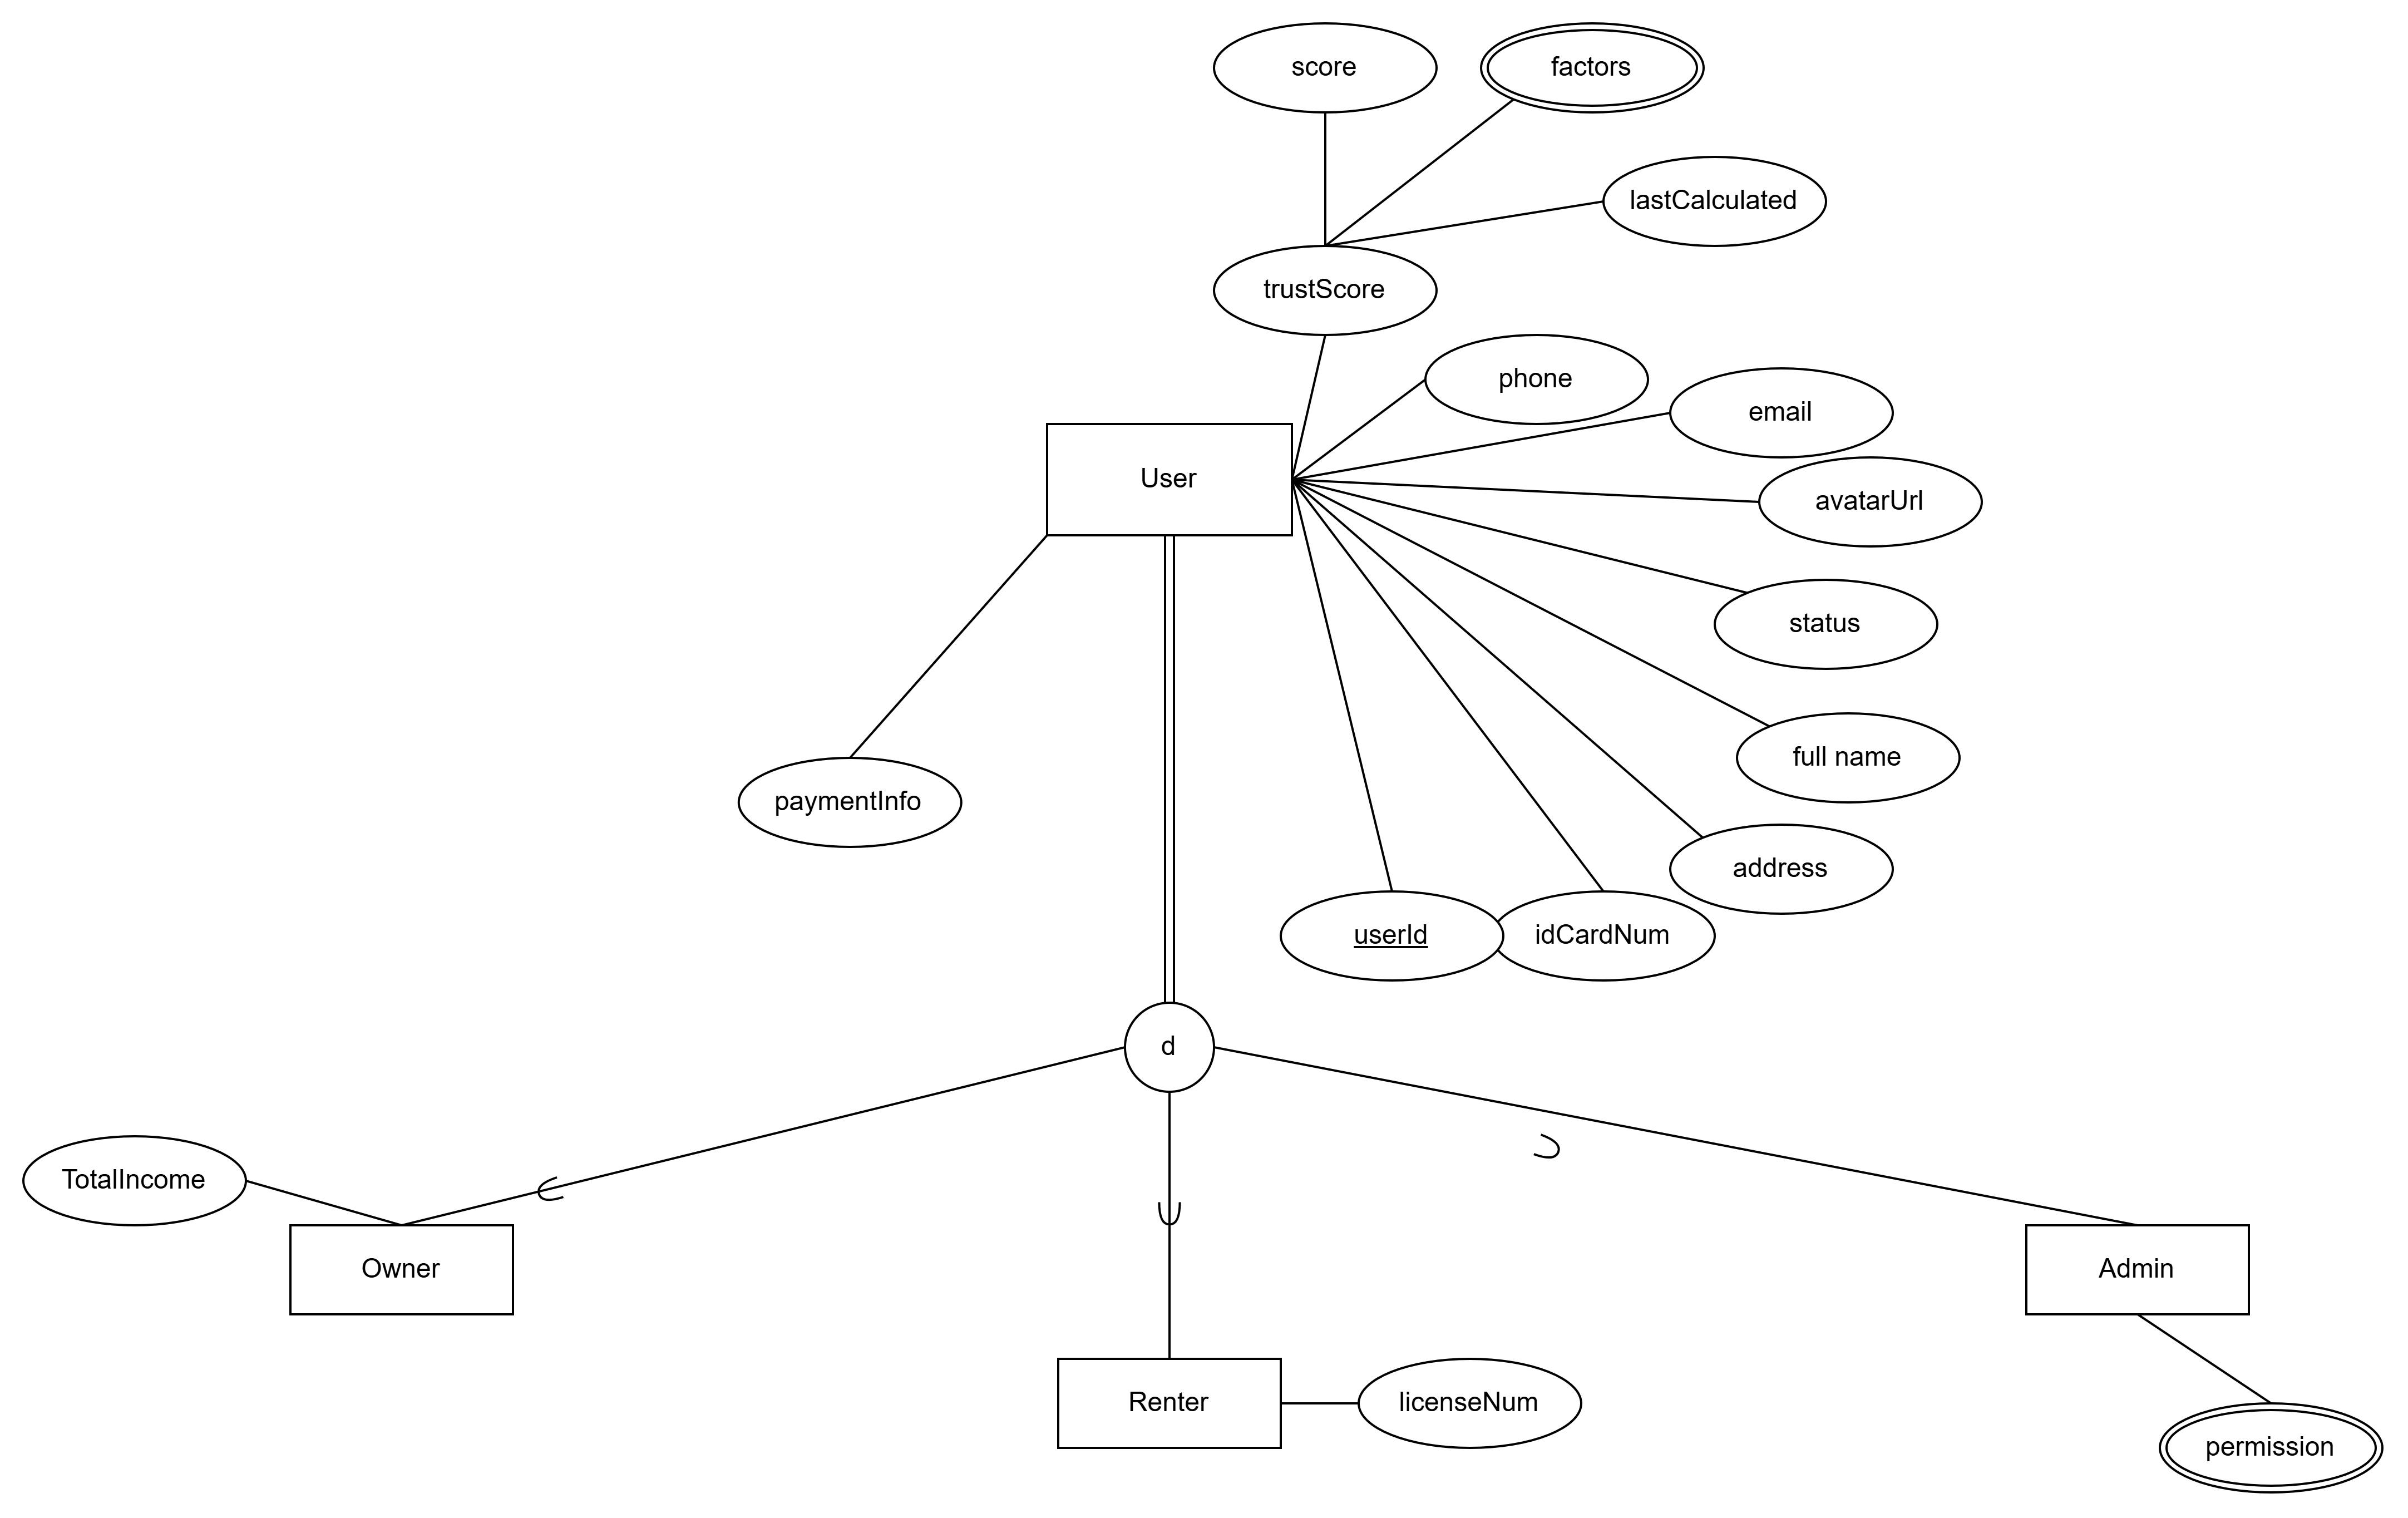
\includegraphics[width=0.6\textwidth]{Images/Design/DB/user.png}
%     \caption{Quan hệ kế thừa giữa users với renters, owners, admins}
%     \label{fig:rel-inheritance}
% \end{figure}

\subsubsection{Quan hệ giữa các thực thể}

\textbf{(1) User -- Notification (1:N)} \\[4pt]
Mỗi \texttt{Notification} phải thuộc về đúng một \texttt{User} (tham gia bắt buộc). 
Một \texttt{User} có thể có không hoặc nhiều thông báo (0..N). 
Triển khai bằng foreign key \texttt{userId} trong bảng \texttt{Notification} với constraint NOT NULL.

\begin{figure}[H]
    \centering
    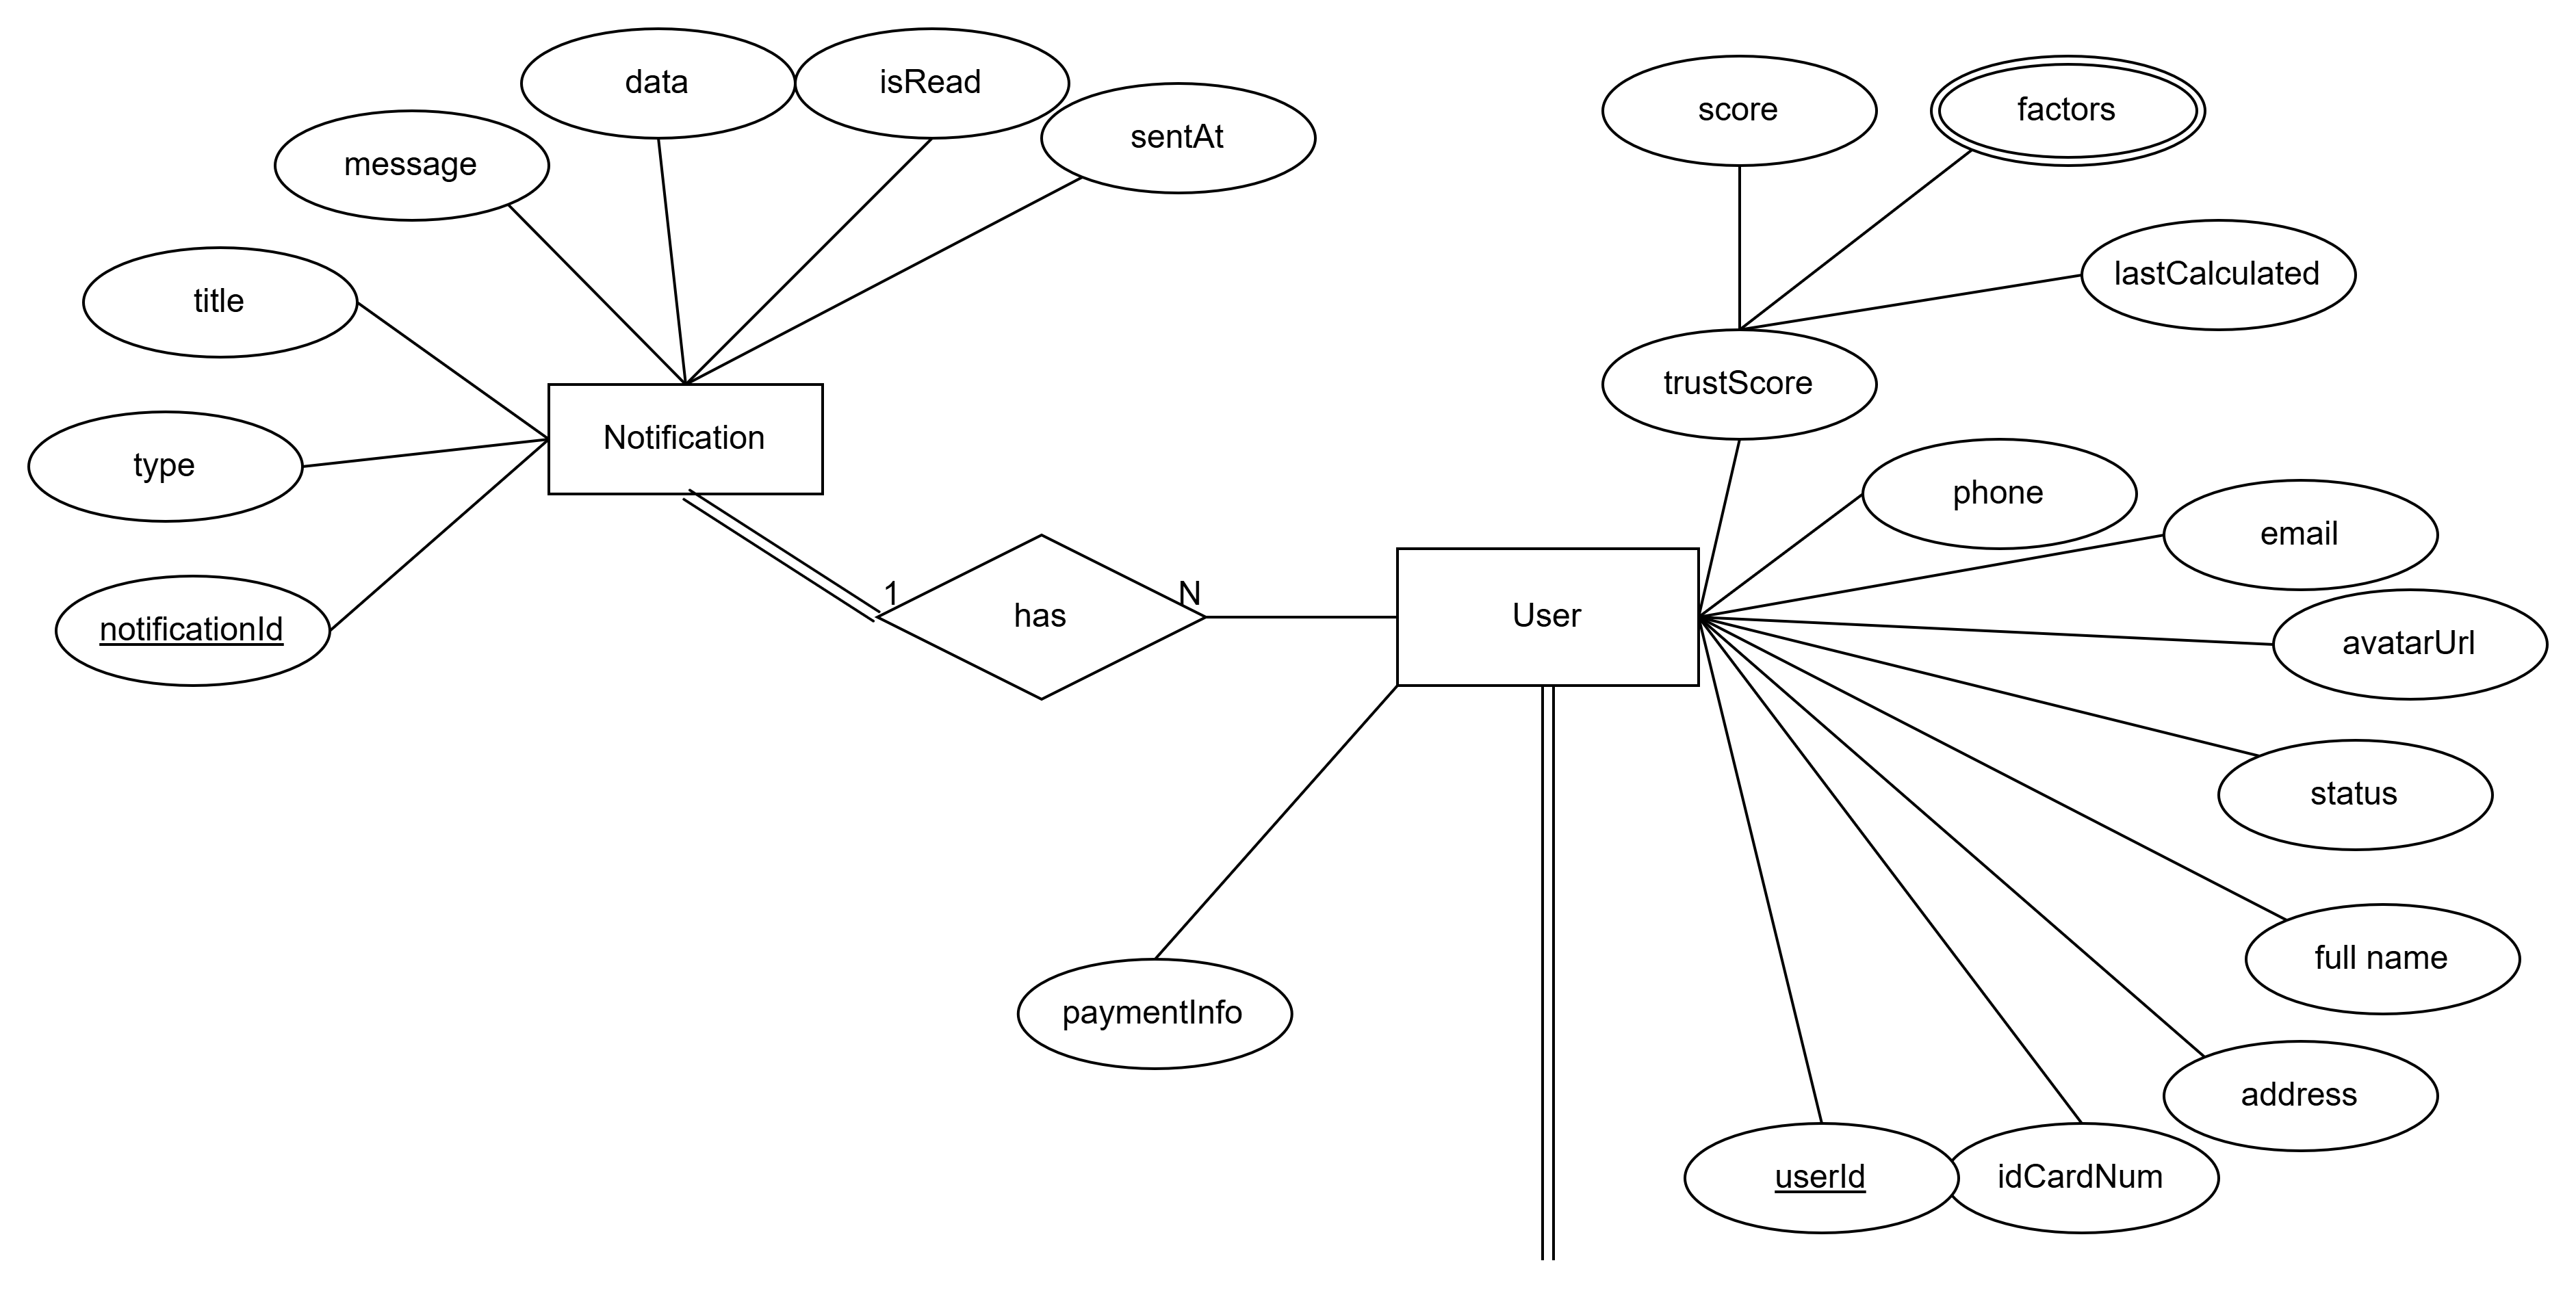
\includegraphics[width=0.8\textwidth]{Images/Design/DB/user-notify.png}
    \caption{Quan hệ giữa \texttt{User} và \texttt{Notification} (1:N)}
    \label{fig:rel-user-notification}
\end{figure}

\vspace{10pt}

\textbf{(2) Admin -- AnalyticsReport (1:N)} \\[4pt]
Mỗi \texttt{AnalyticsReport} được tạo bởi đúng một \texttt{Admin} (tham gia bắt buộc). 
Một \texttt{Admin} có thể tạo nhiều báo cáo hoặc chưa tạo báo cáo nào (0..N). 
Foreign key \texttt{adminId} trong bảng \texttt{AnalyticsReport}.

\begin{figure}[H]
    \centering
    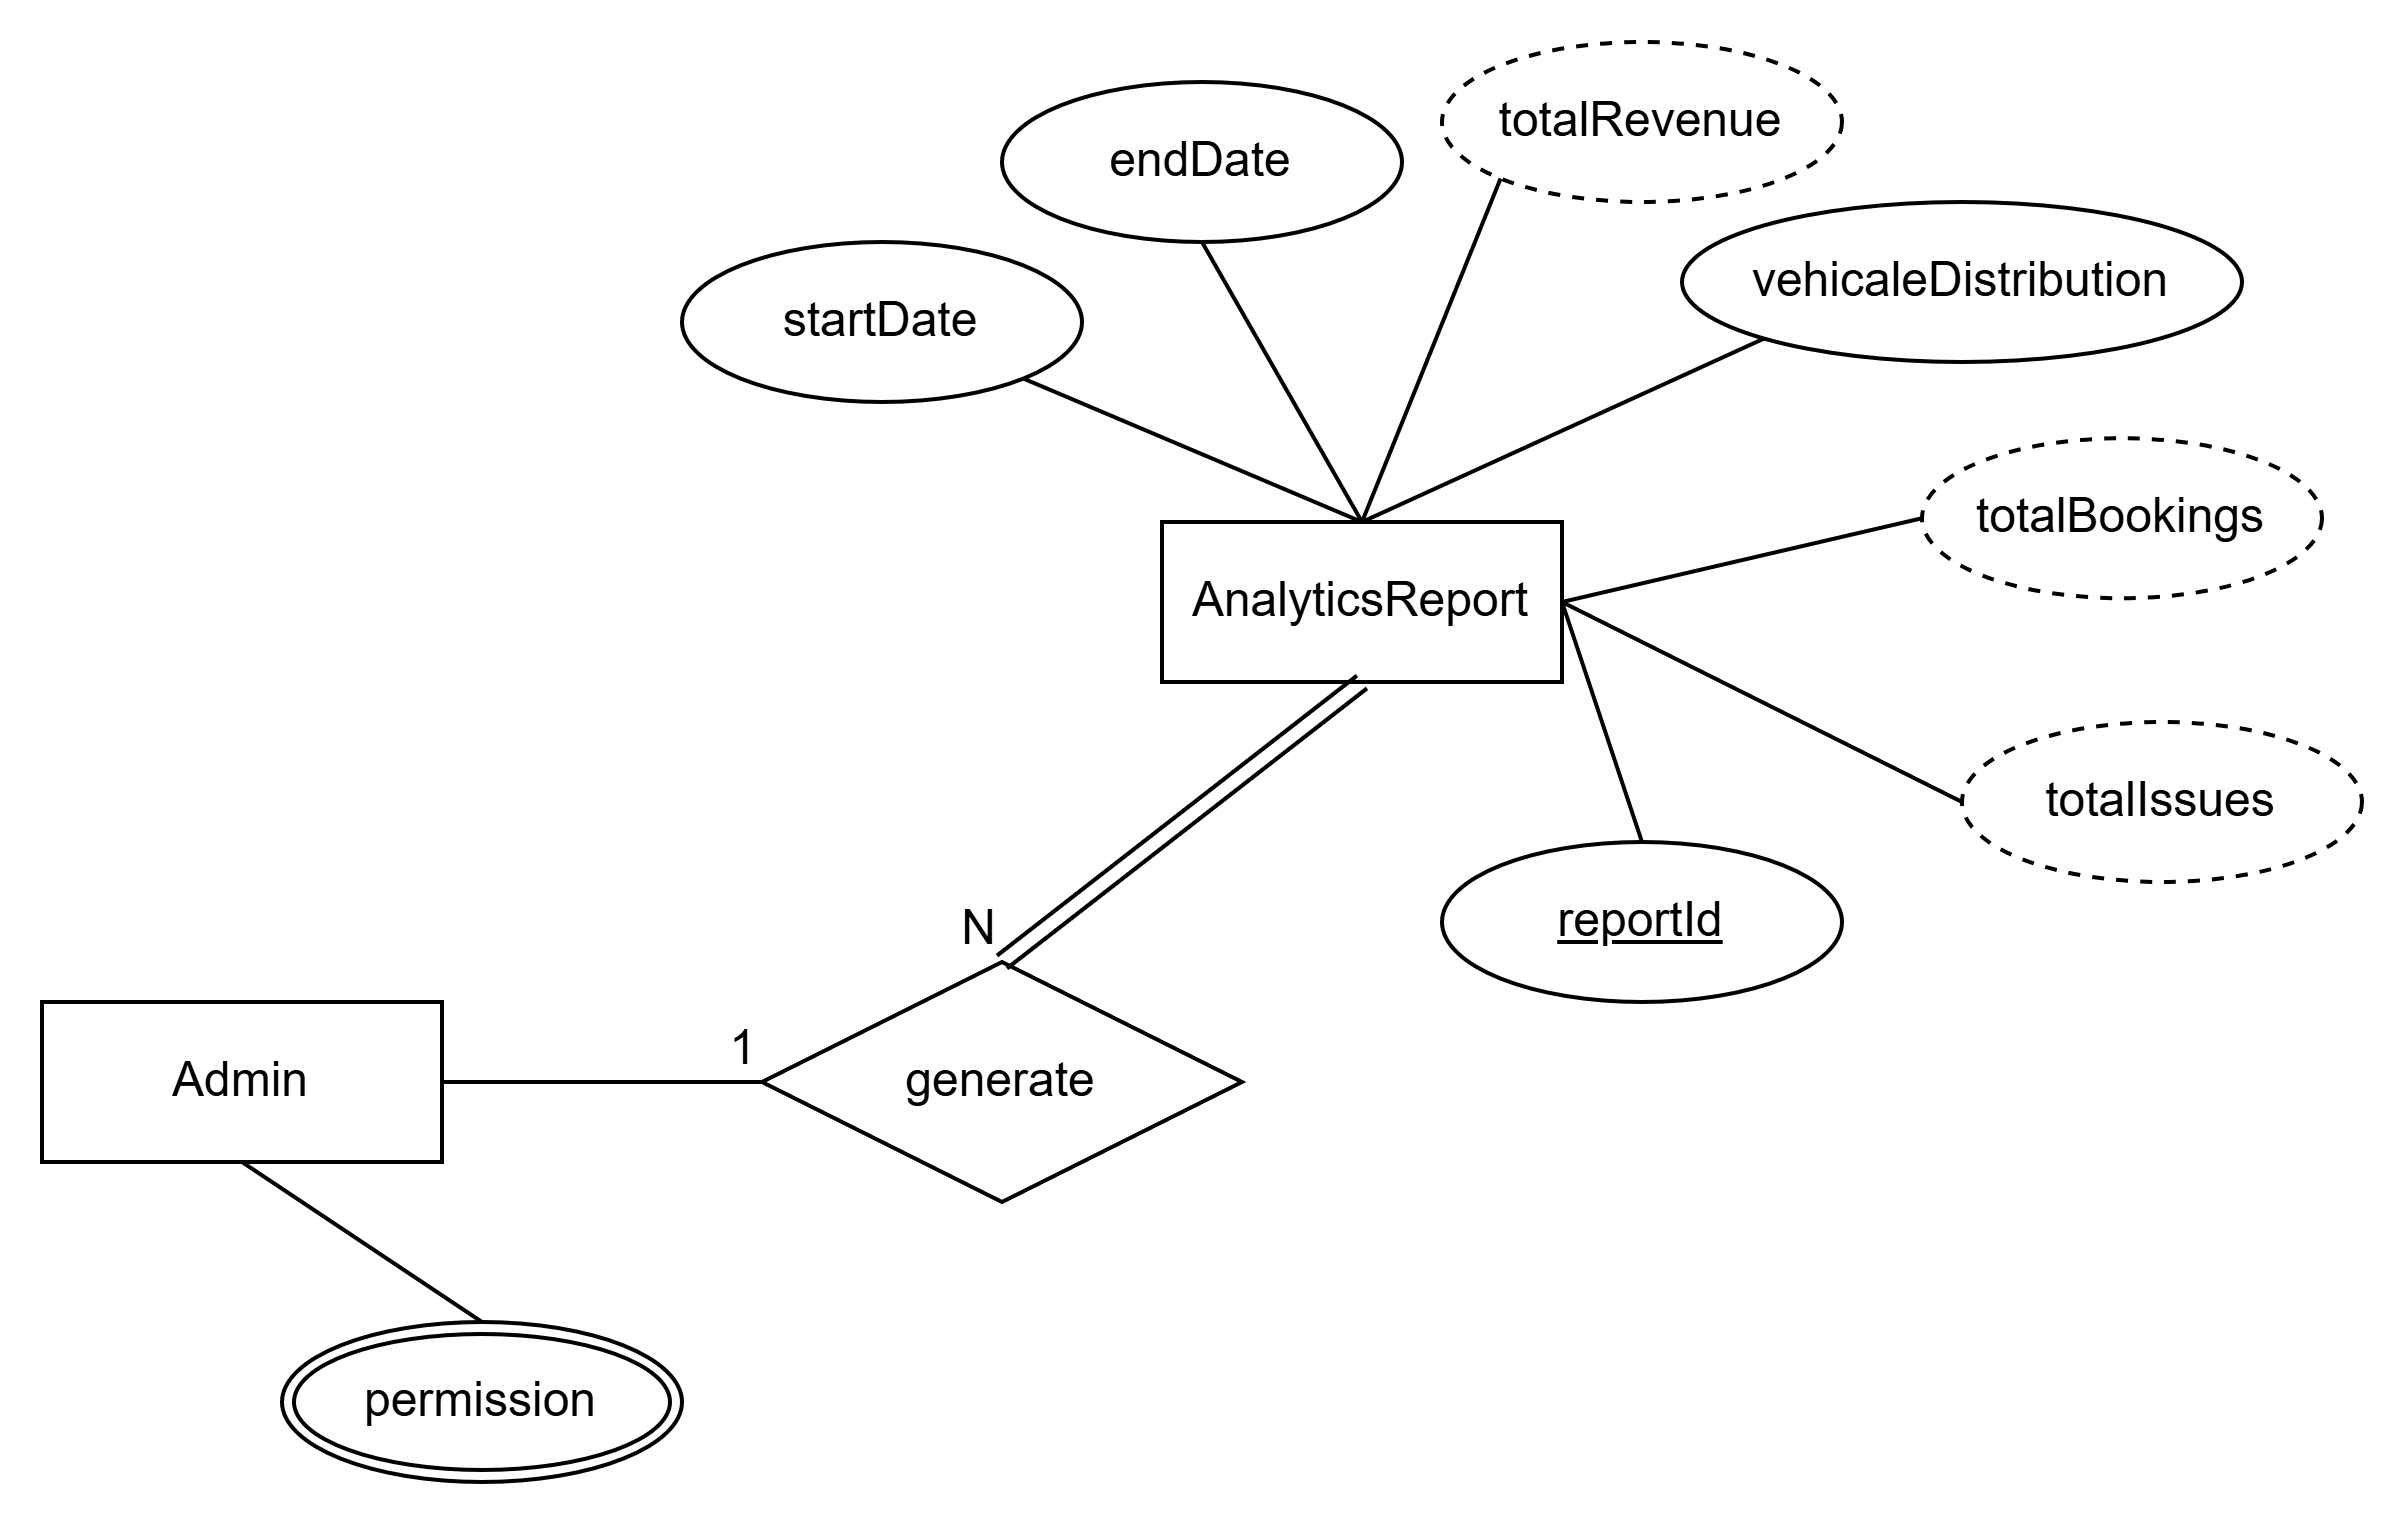
\includegraphics[width=0.8\textwidth]{Images/Design/DB/admin-report.png}
    \caption{Quan hệ giữa \texttt{Admin} và \texttt{AnalyticsReport} (1:N)}
    \label{fig:rel-admin-report}
\end{figure}

\vspace{10pt}

\textbf{(3) Owner -- Vehicle (1:N)} \\[4pt]
Mỗi \texttt{Vehicle} phải thuộc về đúng một \texttt{Owner} (tham gia bắt buộc). 
Một \texttt{Owner} có thể sở hữu nhiều xe hoặc chưa có xe nào (0..N). 
Foreign key \texttt{ownerId} trong bảng \texttt{Vehicle} với constraint NOT NULL.

\begin{figure}[H]
    \centering
    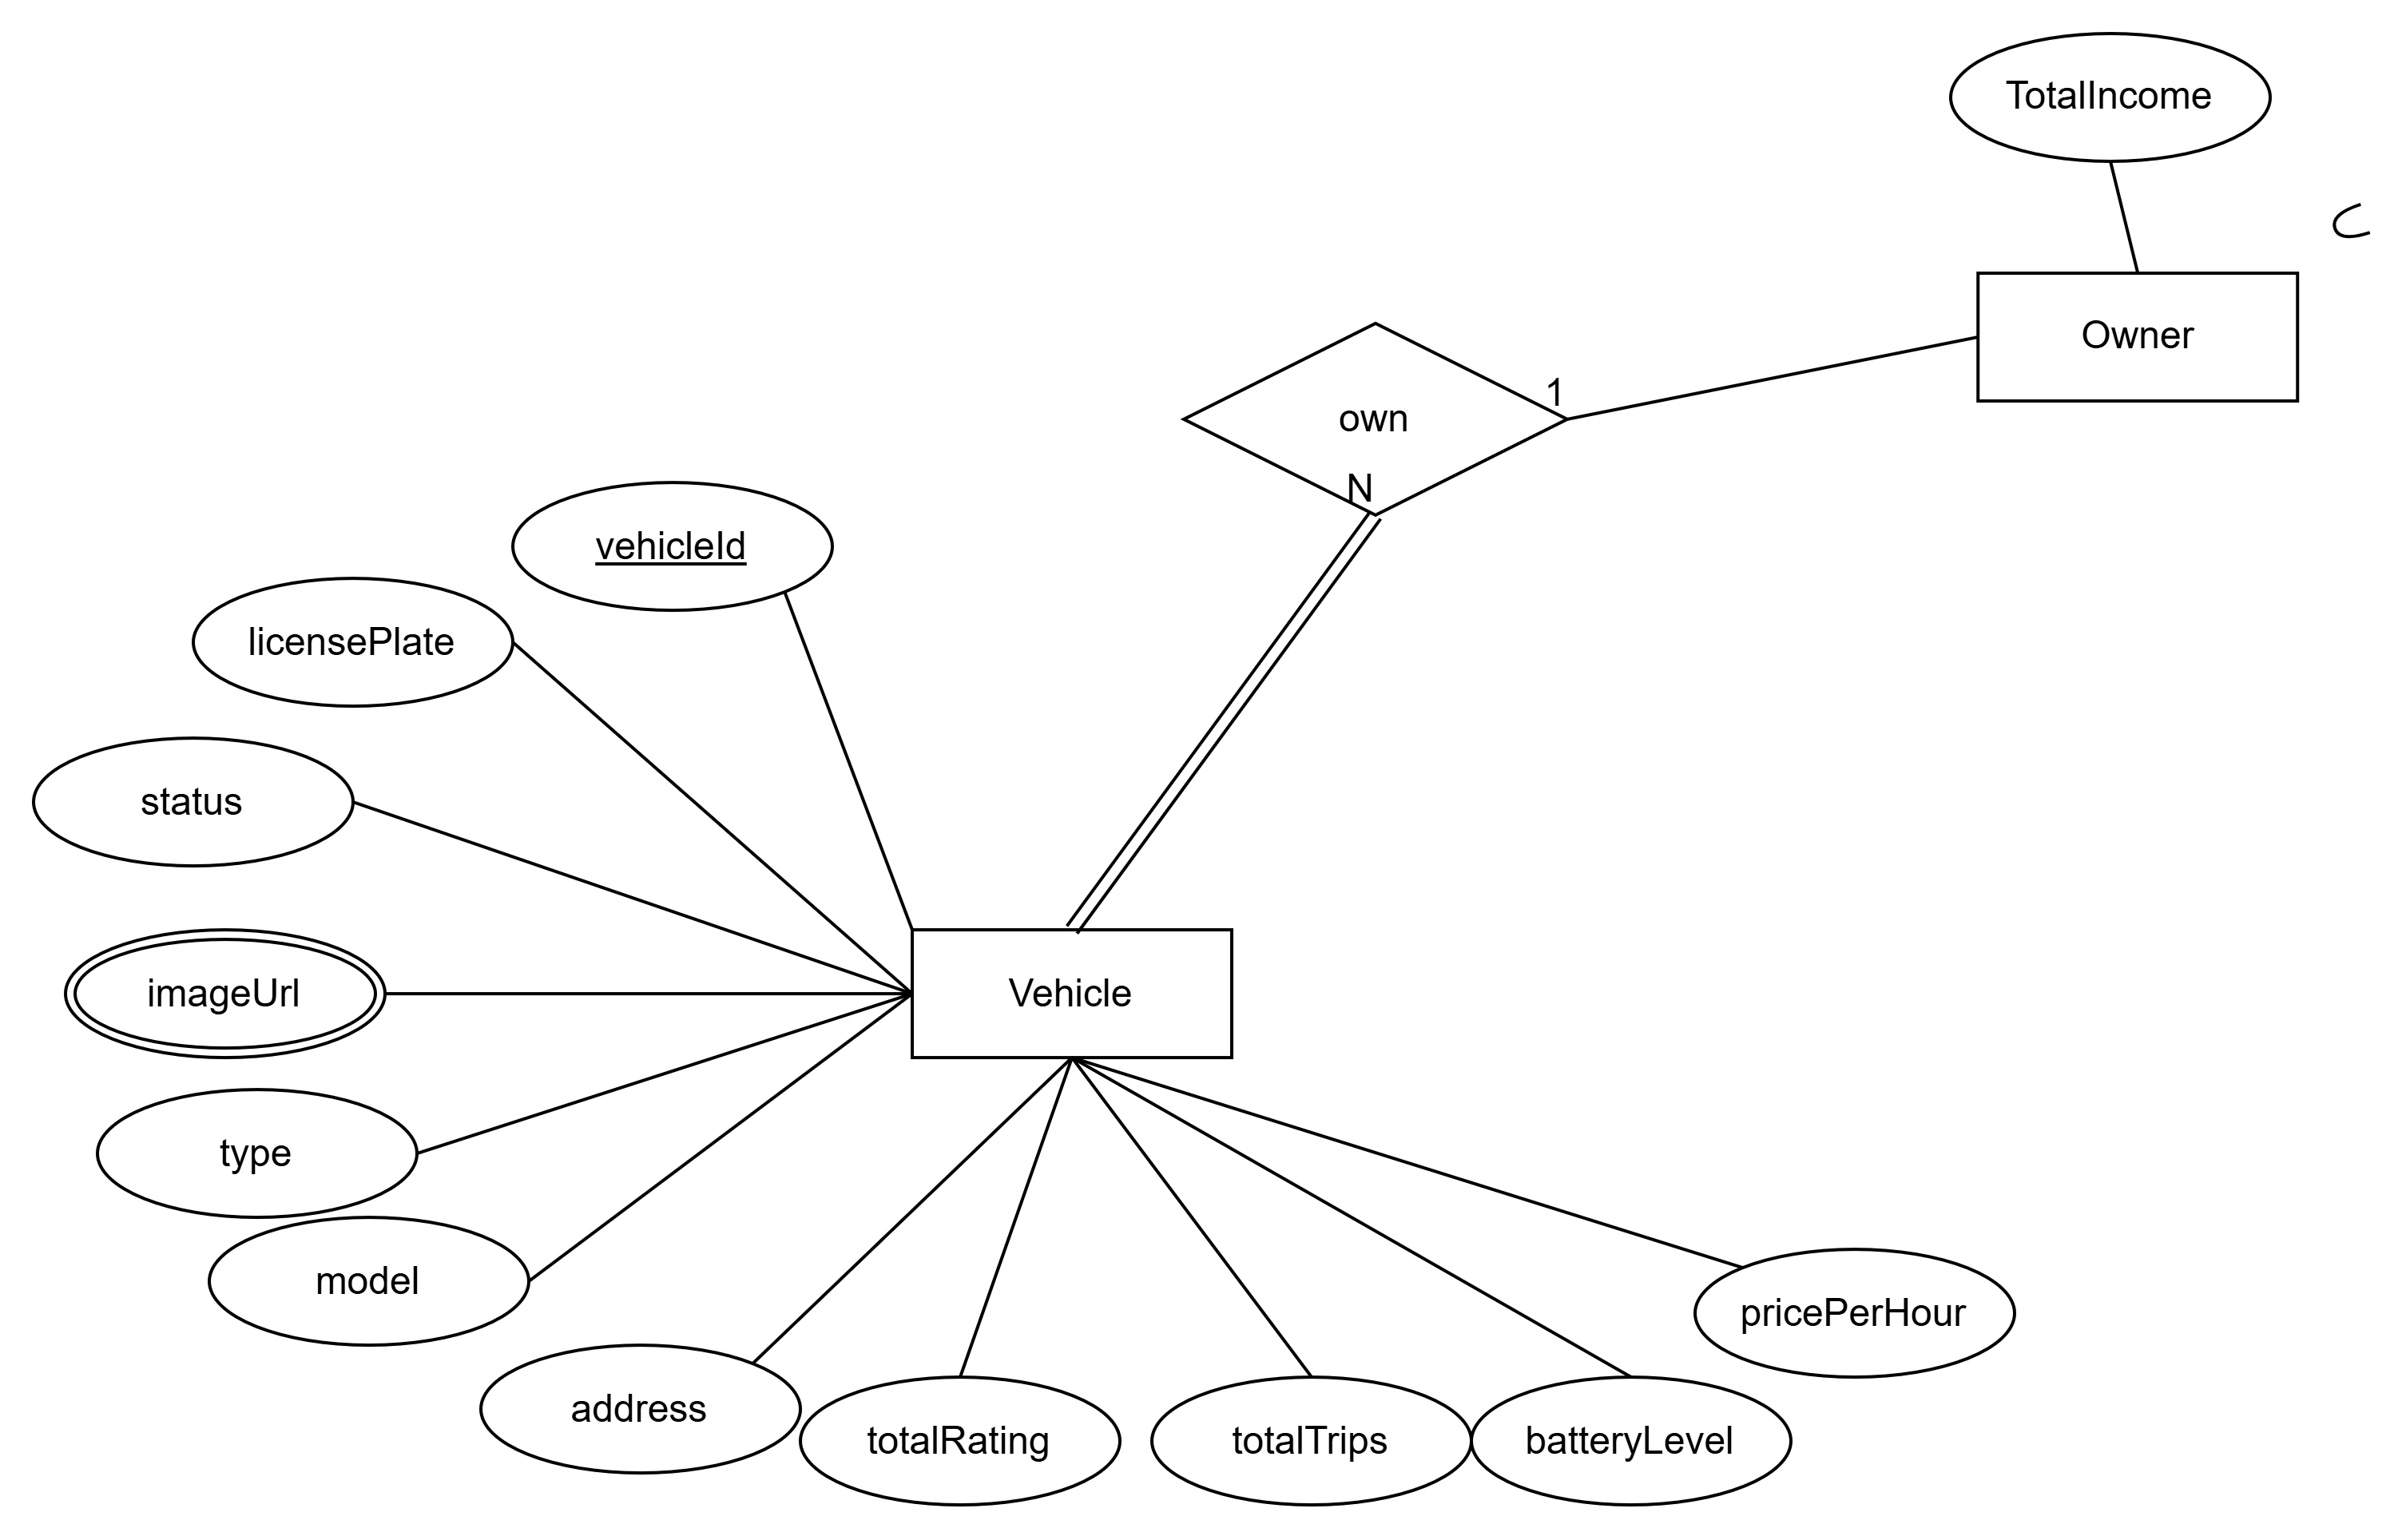
\includegraphics[width=0.8\textwidth]{Images/Design/DB/owner-vehicle.png}
    \caption{Quan hệ giữa \texttt{Owner} và \texttt{Vehicle} (1:N)}
    \label{fig:rel-owner-vehicle}
\end{figure}

\vspace{10pt}

\textbf{(4) Renter -- Booking (1:N)} \\[4pt]
Mỗi \texttt{Booking} được tạo bởi đúng một \texttt{Renter} (tham gia bắt buộc). 
Một \texttt{Renter} có thể tạo nhiều booking hoặc chưa có booking nào (0..N). 
Foreign key \texttt{renterId} trong bảng \texttt{Booking} với constraint NOT NULL.

\begin{figure}[H]
    \centering
    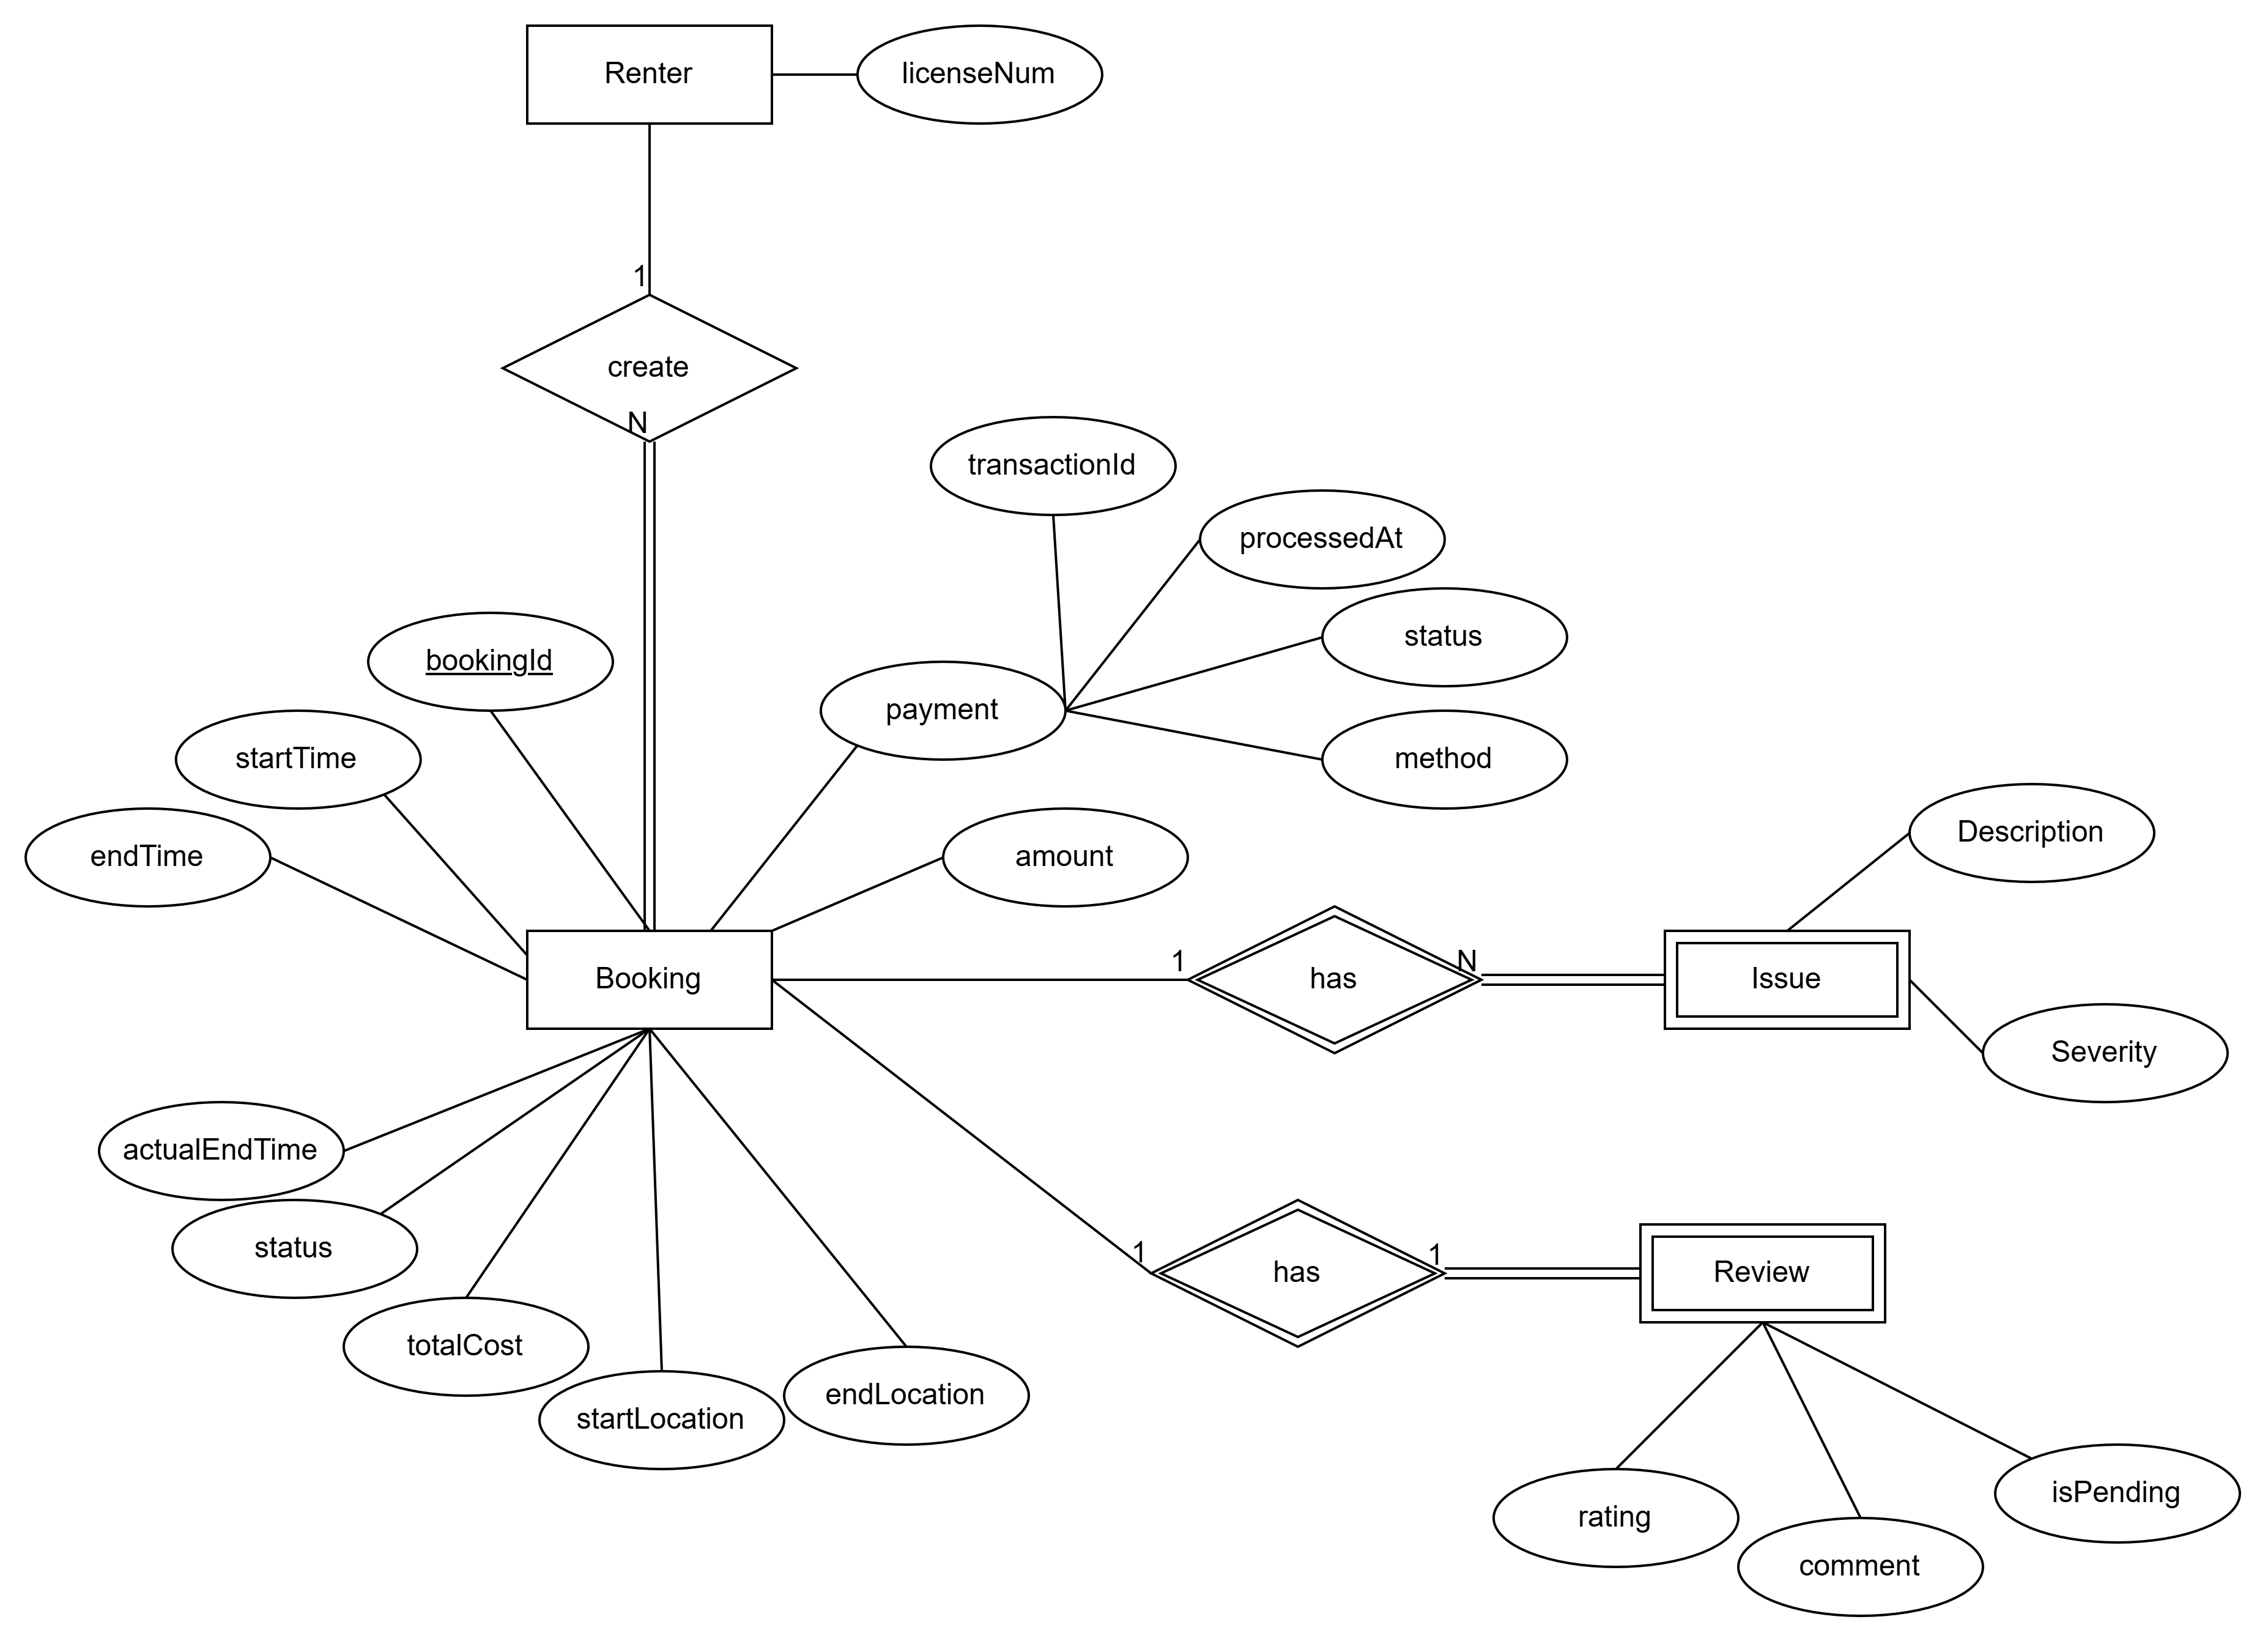
\includegraphics[width=0.8\textwidth]{Images/Design/DB/renter-booking.png}
    \caption{Quan hệ giữa \texttt{Renter} và \texttt{Booking} (1:N)}
    \label{fig:rel-renter-booking}
\end{figure}

\vspace{10pt}

\textbf{(5) Vehicle -- Booking (1:N)} \\[4pt]
Mỗi \texttt{Booking} phải gắn với đúng một \texttt{Vehicle} (tham gia bắt buộc). 
Một \texttt{Vehicle} có thể có nhiều booking hoặc chưa được thuê (0..N). 
Foreign key \texttt{vehicleId} trong bảng \texttt{Booking} với constraint NOT NULL. 
Hỗ trợ kiểm tra xung đột thời gian thuê xe.

\begin{figure}[H]
    \centering
    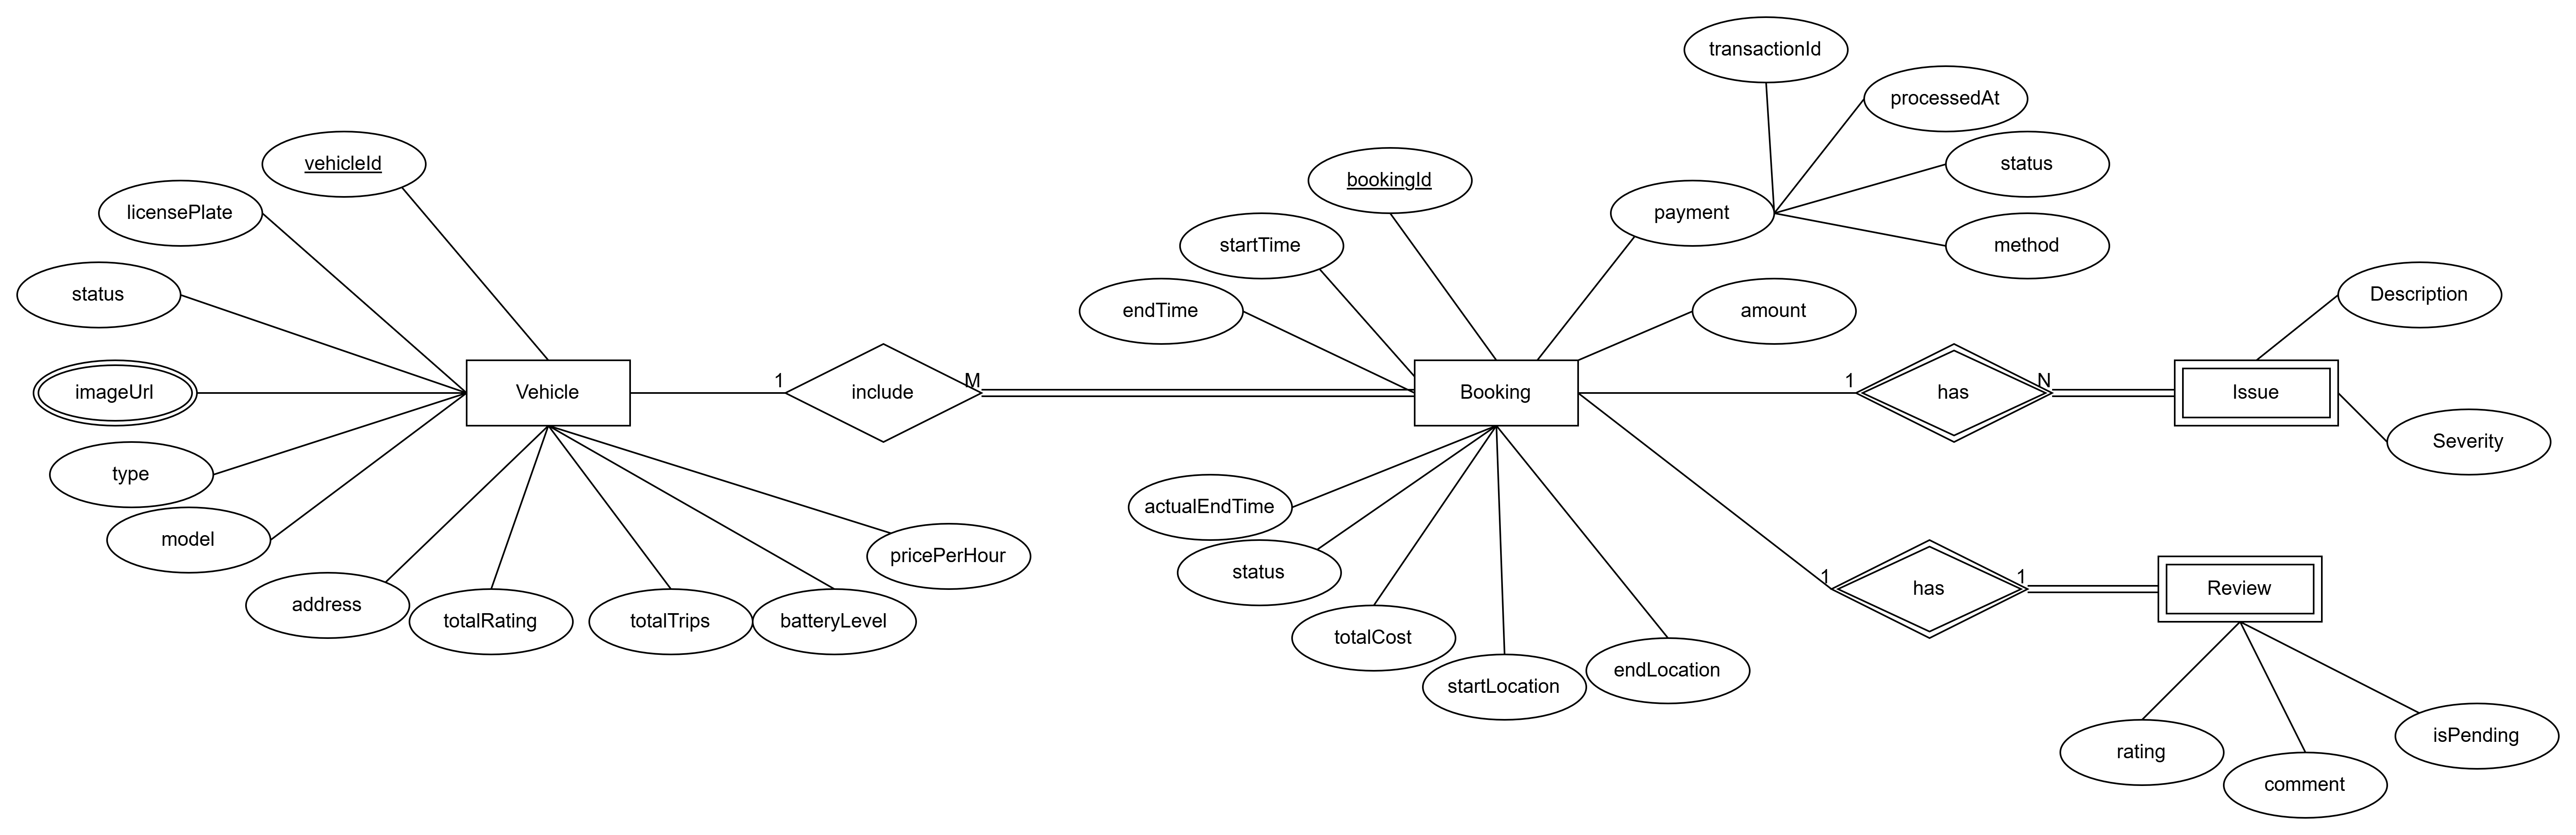
\includegraphics[width=1.0\textwidth]{Images/Design/DB/vehicle-booking.png}
    \caption{Quan hệ giữa \texttt{Vehicle} và \texttt{Booking} (1:N)}
    \label{fig:rel-vehicle-booking}
\end{figure}

\vspace{10pt}

\textbf{(6) Booking} \\[4pt]
\begin{figure}[H]
    \centering
    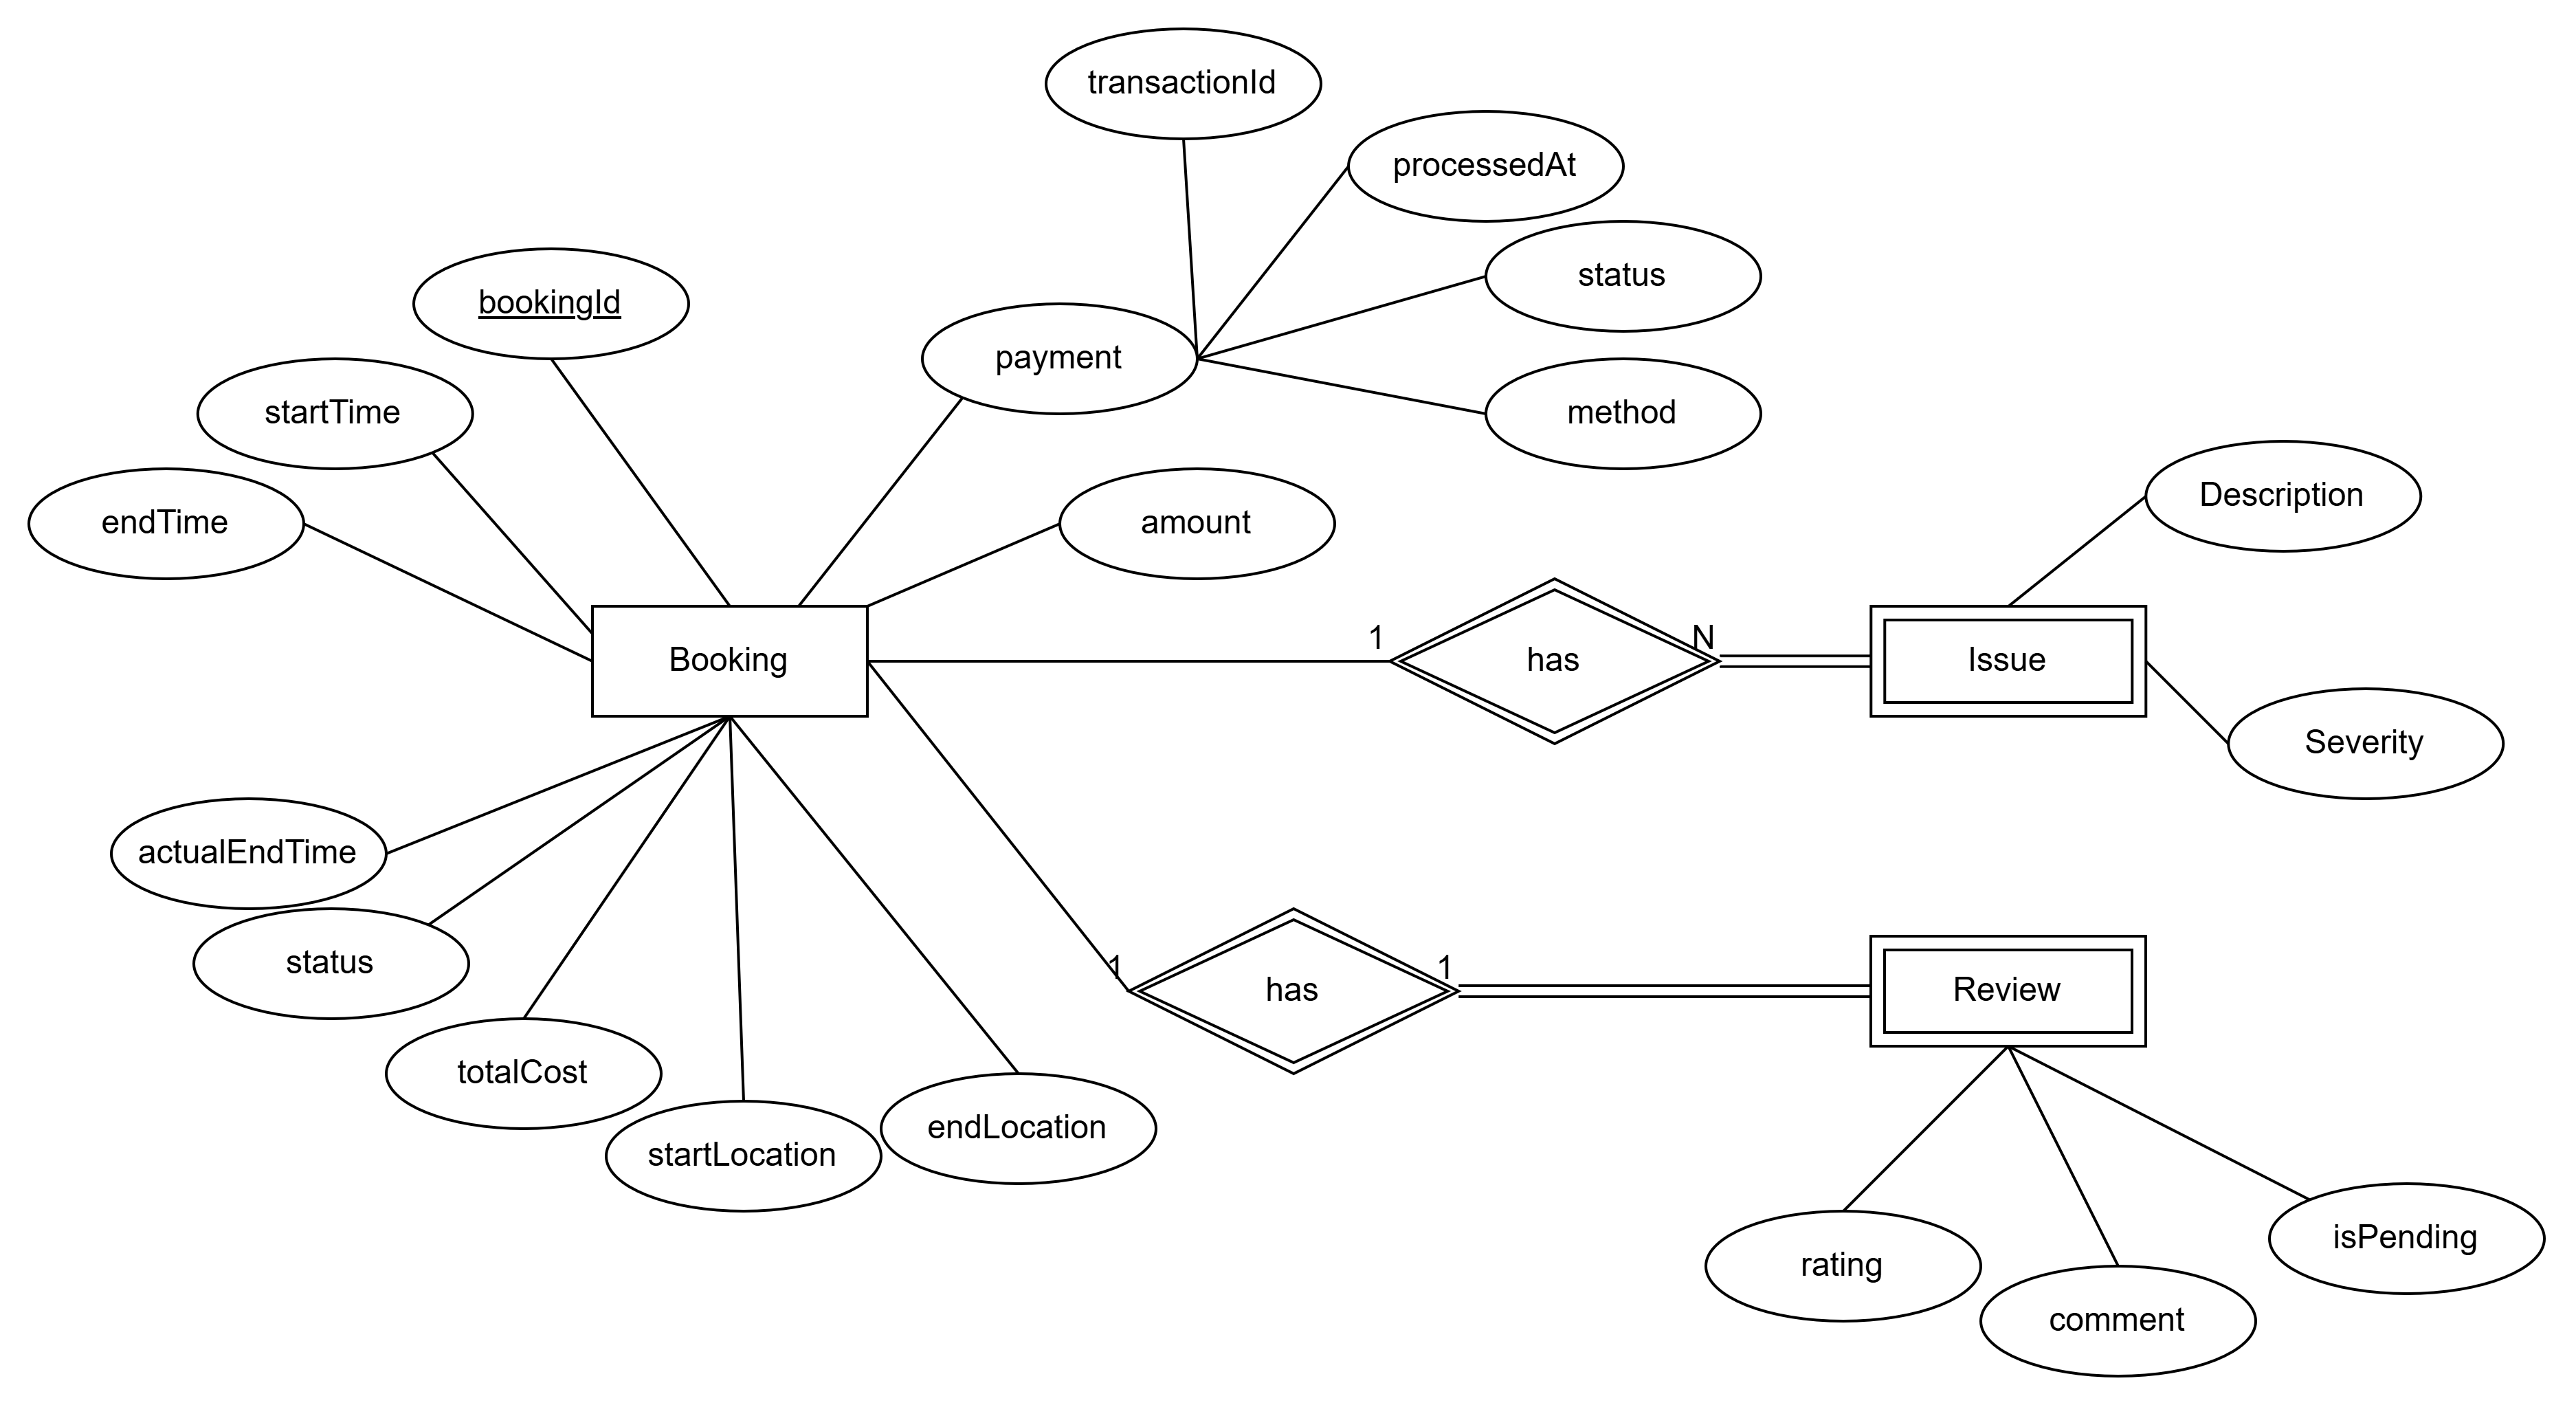
\includegraphics[width=0.8\textwidth]{Images/Design/DB/booking-payment.png}
    \caption{Quan hệ giữa \texttt{Booking} và \texttt{Payment} (1:N)}
    \label{fig:rel-booking-payment}
\end{figure}

\begin{itemize}
    \item[(6.1)] \textbf{Booking -- Review (1:1)} \\[4pt]
    Mỗi \texttt{Review} phải gắn với đúng một \texttt{Booking} (tham gia bắt buộc). 
    Mỗi \texttt{Booking} có đúng một \texttt{Review} (tham gia bắt buộc, quan hệ 1:1). 
    Foreign key \texttt{bookingId} trong bảng \texttt{Review} với constraint NOT NULL và UNIQUE để đảm bảo mỗi booking chỉ có một đánh giá.
    \item[(6.2)] \textbf{Booking -- Issue (1:N)} \\[4pt]
    Một \texttt{Booking} có thể phát sinh nhiều sự cố.  
    Một \texttt{Issue} phải thuộc về đúng một \texttt{Booking}.
\end{itemize}

\textbf{(8) Mối quan hệ kế thừa giữa các thực thể người dùng hệ thống} \\[4pt]
Mỗi \texttt{User} phải thuộc \textbf{đúng 1} trong 3 loại: \texttt{Renter}, \texttt{Owner}, hoặc \texttt{Admin}.
\texttt{Renter}, \texttt{Owner}, \texttt{Admin} chia sẻ \texttt{userId} (FK → User.id)

\begin{figure}[H]
    \centering
    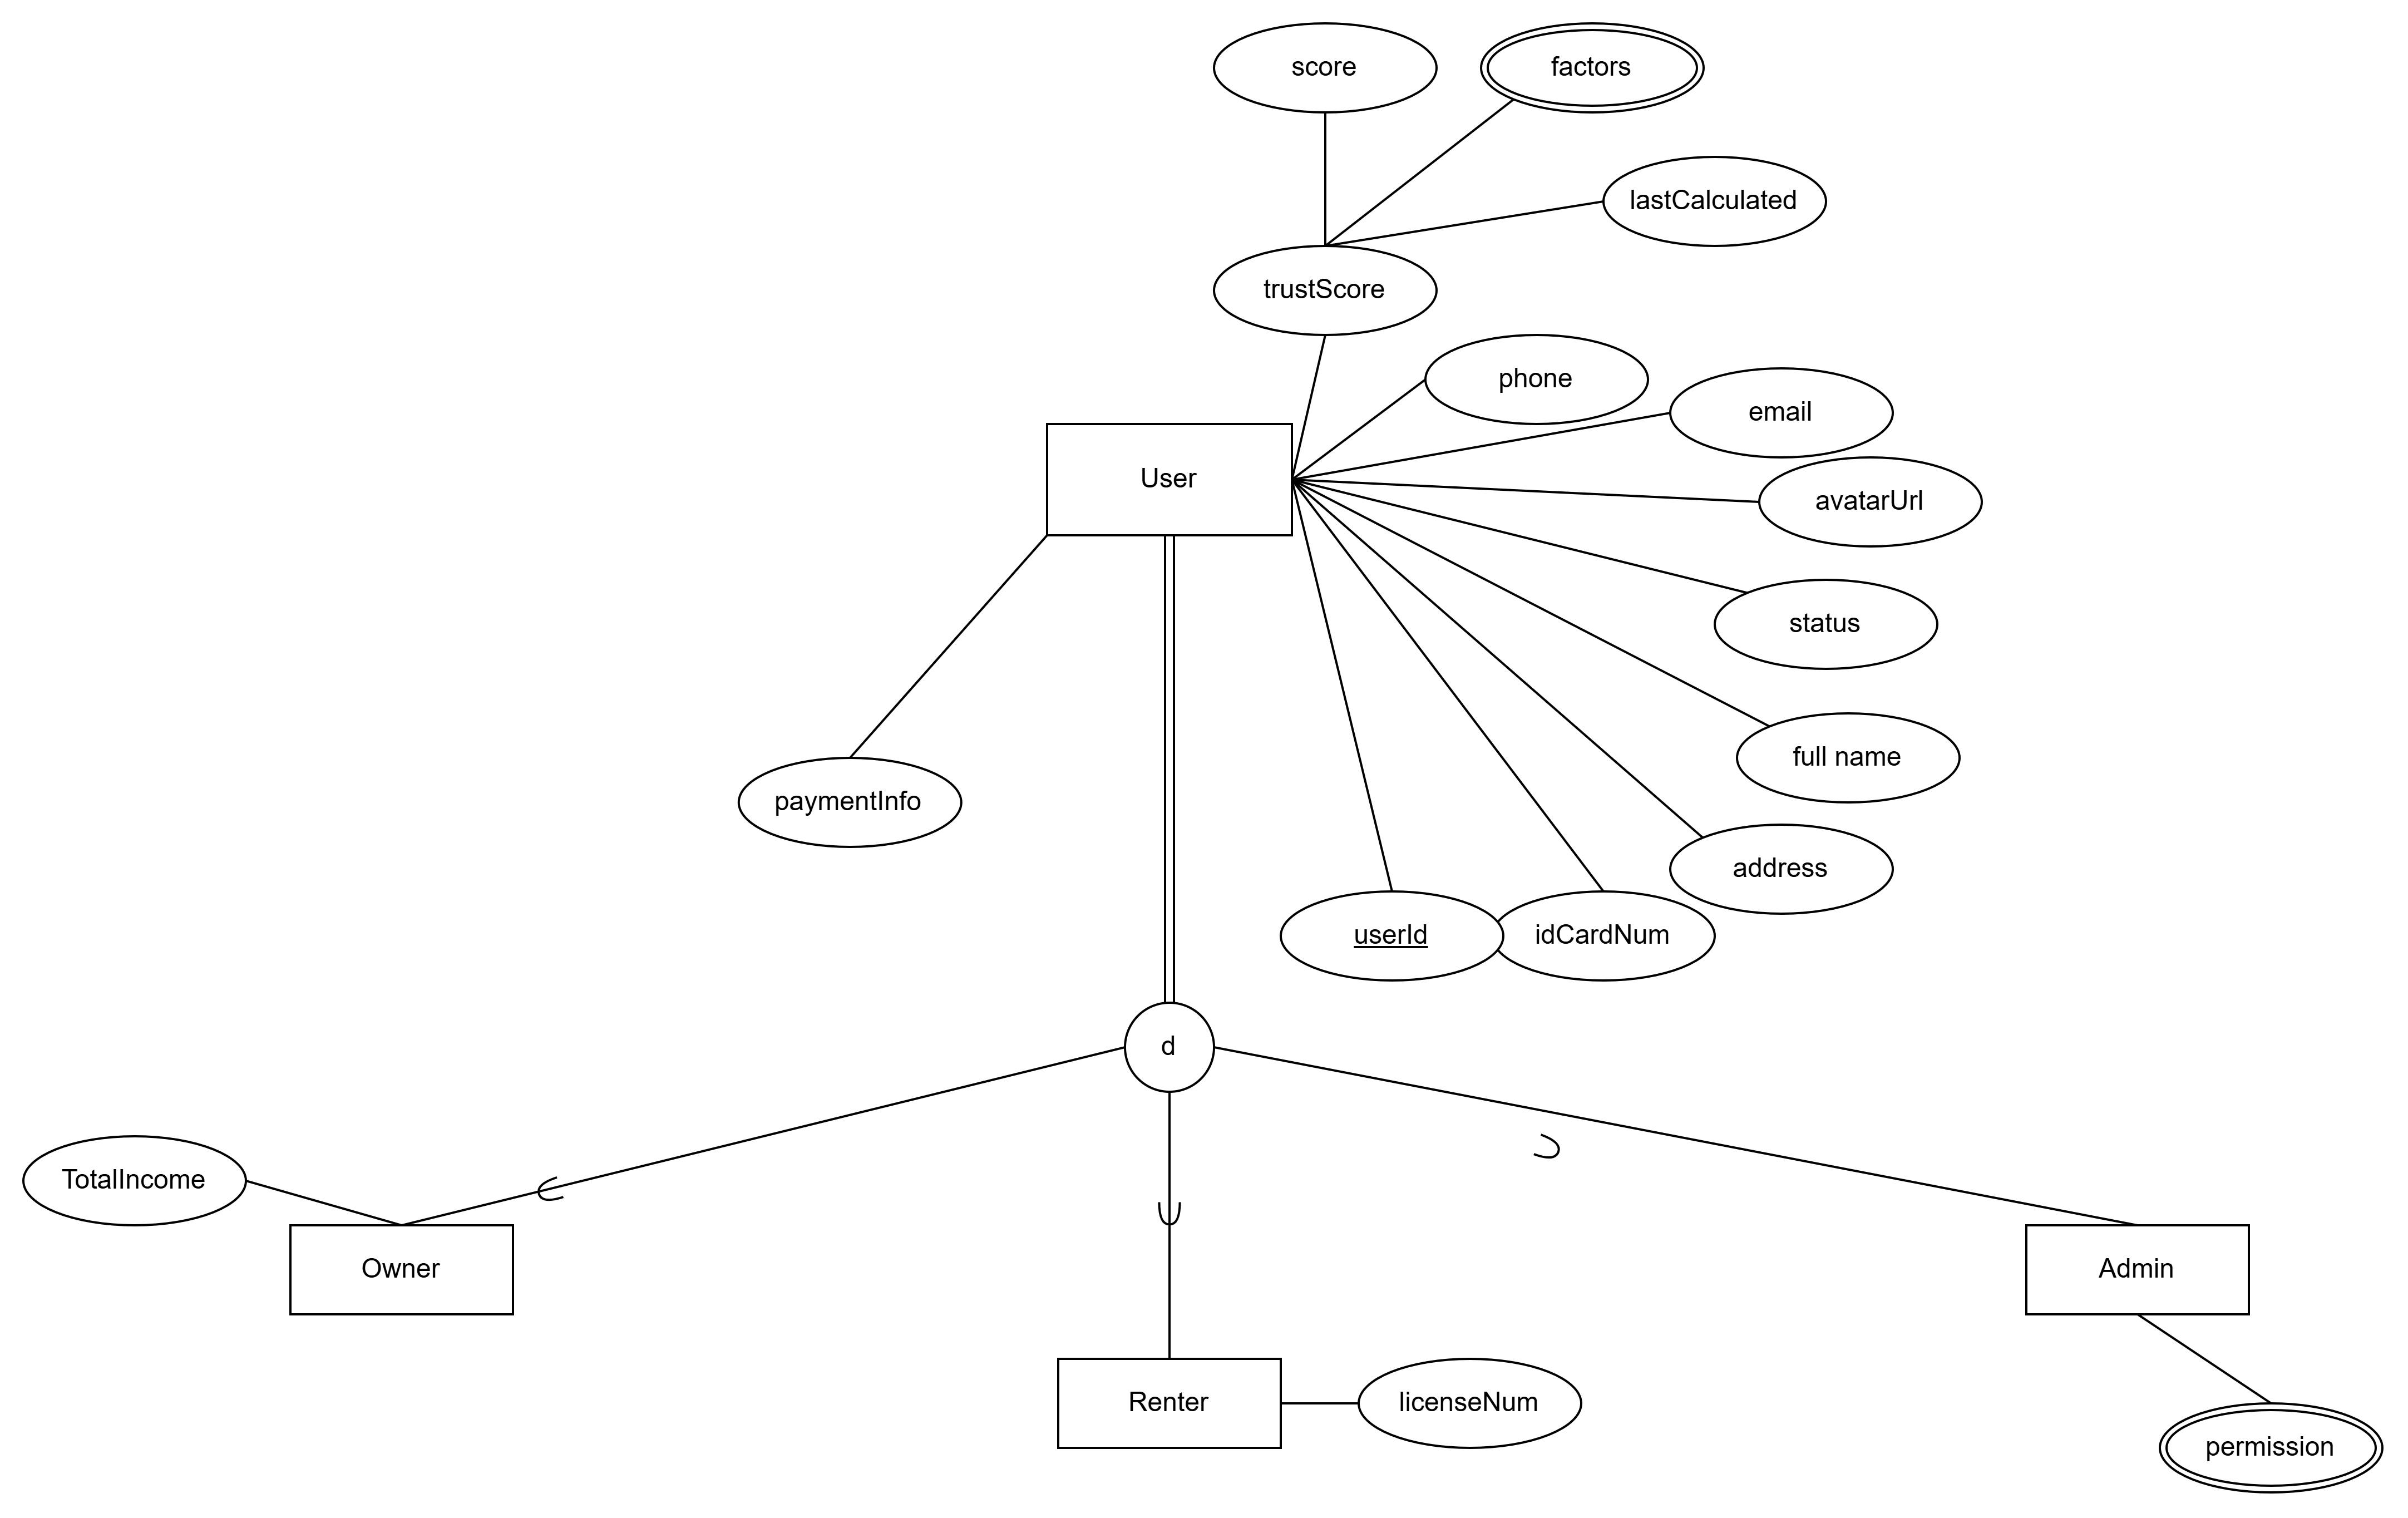
\includegraphics[width=0.8\textwidth]{Images/Design/DB/user.png}
    \caption{Quan hệ kế thừa giữa User với Renter, User, Admin}
    \label{fig:rel-inheritance}
\end{figure}

% \subsubsection*{Kế thừa (Inheritance)}

% Hệ thống sử dụng \textbf{discrete, mandatory inheritance}:
% \begin{itemize}[leftmargin=*]
%     \item Mỗi \texttt{User} phải thuộc \textbf{đúng 1} trong 3 loại: \texttt{Renter}, \texttt{Owner}, hoặc \texttt{Admin}
%     \item Triển khai: Table Per Concrete Class hoặc Single Table Inheritance với trường \texttt{role}
%     \item \texttt{Renter}, \texttt{Owner}, \texttt{Admin} chia sẻ \texttt{userId} (FK → User.id)
% \end{itemize}

% \subsubsection{Ràng buộc toàn vẹn}

% \begin{enumerate}[leftmargin=*]
%     \item \textbf{Notification}: Mỗi notification phải liên kết đến đúng 1 user (NOT NULL \texttt{userId})
%     \item \textbf{Vehicle ownership}: Mỗi vehicle phải có owner (NOT NULL \texttt{ownerId})
%     \item \textbf{Booking}: Mỗi booking phải có renter và vehicle (NOT NULL \texttt{renterId}, \texttt{vehicleId})
%     \item \textbf{Payment}: Mỗi payment phải gắn với 1 booking (NOT NULL \texttt{bookingId})
%     \item \textbf{Review}: Mỗi review phải gắn với 1 booking (NOT NULL \texttt{bookingId}, UNIQUE constraint)
%     \item \textbf{User role}: Mỗi user phải có \texttt{role} $\in$ \{renter, owner, admin\}
%     \item \textbf{Vehicle location}: \texttt{latitude} $\in$ [-90, 90], \texttt{longitude} $\in$ [-180, 180]
%     \item \textbf{Trust score}: \texttt{score} $\in$ [0, 100], \texttt{factors} là JSON array
%     \item \textbf{Booking time}: \texttt{startTime} $ \leqq $ \texttt{endTime}, \texttt{actualEndTime} $\geqq$ \texttt{endTime}
%     \item \textbf{Payment amount}: \texttt{amount} > 0
% \end{enumerate}

% \paragraph{Index và tối ưu hóa}

% \begin{itemize}[leftmargin=*]
%     \item \textbf{Spatial index}: \texttt{CREATE INDEX idx\_vehicle\_location ON vehicles USING GIST (location)}
%     \item \textbf{User queries}: Index trên \texttt{email}, \texttt{phone}, \texttt{status}
%     \item \textbf{Booking queries}: Composite index trên \texttt{(renterId, status)}, \texttt{(vehicleId, startTime)}
%     \item \textbf{Payment queries}: Index trên \texttt{bookingId}, \texttt{status}, \texttt{processedAt}
%     \item \textbf{Full-text search}: Index trên \texttt{Vehicle.model}, \texttt{Vehicle.type}
% \end{itemize}

% \subsection{Yêu cầu dữ liệu}

% \subsubsection{Tổng quan các thực thể dữ liệu}

% Hệ thống chia sẻ xe máy điện P2P quản lý mười thực thể dữ liệu chính, được phân loại thành ba nhóm: dữ liệu chủ (master data) đại diện cho các tham gia viên và tài nguyên hệ thống, dữ liệu giao dịch (transactional data) ghi lại các hoạt động vận hành, và dữ liệu phân tích (analytical data) hỗ trợ giám sát và cải tiến hệ thống.

% \textbf{Dữ liệu chủ} bao gồm User (người tham gia hệ thống với thông tin xác thực và hồ sơ), Renter (chuyên biệt hóa của User với lịch sử thuê và sở thích), Owner (chuyên biệt hóa của User với quyền sở hữu xe và thông tin tài khoản tài chính), Admin (quản trị viên hệ thống với quyền nâng cao), và Vehicle (xe máy điện khả dụng để chia sẻ, bao gồm thông số kỹ thuật và trạng thái hiện tại). Các thực thể này có tần suất cập nhật thấp nhưng tầm quan trọng tham chiếu cao, phục vụ như các mục tiêu khóa ngoại cho các bản ghi giao dịch.

% \textbf{Dữ liệu giao dịch} bao gồm Booking (thỏa thuận thuê xe giữa người thuê và chủ xe, bao gồm khoảng thời gian và tính toán chi phí), Payment (các giao dịch tài chính liên quan đến booking, hỗ trợ nhiều phương thức thanh toán và theo dõi trạng thái), và Review (đánh giá sau khi thuê đóng góp vào tính toán điểm tin cậy). Các thực thể này trải qua khối lượng chèn cao trong quá trình hoạt động hệ thống, tạo thành hồ sơ vận hành cho phép phân tích kinh doanh.

% \textbf{Dữ liệu phân tích và hỗ trợ vận hành} bao gồm Notification (cảnh báo thời gian thực và thông điệp hệ thống cho người dùng) và AnalyticsReport (thống kê tổng hợp được tạo bởi quản trị viên để giám sát hiệu suất hệ thống). Mặc dù không trực tiếp tham gia vào quy trình thuê xe cốt lõi, các thực thể này hỗ trợ trải nghiệm người dùng và các chức năng quản lý hệ thống.

% \subsubsection{Ước tính khối lượng dữ liệu}

% Dự báo khối lượng cung cấp thông tin cho việc lập kế hoạch dung lượng cơ sở dữ liệu và các chiến lược tối ưu hóa truy vấn. Các ước tính xuất phát từ định nghĩa phạm vi dự án: triển khai ban đầu trong 2-3 cộng đồng hỗ trợ khoảng 30-50 xe, 100-150 người dùng hoạt động và 300-500 giao dịch thuê trong giai đoạn thử nghiệm.

% \begin{table}[h]
% \centering
% \caption{Dự báo khối lượng dữ liệu ban đầu (giai đoạn thử nghiệm 6 tháng)}
% \begin{tabular}{|l|r|r|l|}
% \hline
% \textbf{Thực thể} & \textbf{Ban đầu} & \textbf{Tốc độ tăng} & \textbf{Tổng 6 tháng} \\
% \hline
% User & 100 & 10-15/tháng & 150-180 \\
% \hline
% Renter & 80 & 8-12/tháng & 120-150 \\
% \hline
% Owner & 35 & 2-3/tháng & 45-55 \\
% \hline
% Admin & 3 & 0/tháng & 3-5 \\
% \hline
% Vehicle & 40 & 3-5/tháng & 55-65 \\
% \hline
% Booking & 50 & 60-80/tháng & 400-500 \\
% \hline
% Payment & 100 & 120-160/tháng & 800-1,000 \\
% \hline
% Review & 30 & 40-60/tháng & 270-350 \\
% \hline
% Notification & 200 & 300-500/tháng & 2,000-3,200 \\
% \hline
% AnalyticsReport & 0 & 4-8/tháng & 24-48 \\
% \hline
% \end{tabular}
% \end{table}

% Ước tính dung lượng lưu trữ tính đến dữ liệu văn bản, metadata JSON và tham chiếu hình ảnh:

% \begin{itemize}[leftmargin=*]
%     \item \textbf{Thực thể người dùng} (User, Renter, Owner, Admin): Trung bình 2 KB/bản ghi (các trường văn bản, dữ liệu hồ sơ, JSON điểm tin cậy) $\times$ 180 người dùng = 360 KB
%     \item \textbf{Thực thể xe}: Trung bình 5 KB/bản ghi (thông số kỹ thuật, dữ liệu vị trí, tham chiếu hình ảnh) $\times$ 65 xe = 325 KB
%     \item \textbf{Thực thể đặt xe}: Trung bình 1.5 KB/bản ghi (timestamps, tọa độ vị trí, giá) $\times$ 500 bookings = 750 KB
%     \item \textbf{Thực thể thanh toán}: Trung bình 1 KB/bản ghi (dữ liệu giao dịch) $\times$ 1,000 payments = 1 MB
%     \item \textbf{Thực thể đánh giá}: Trung bình 2 KB/bản ghi (xếp hạng, văn bản bình luận) $\times$ 350 reviews = 700 KB
%     \item \textbf{Thực thể thông báo}: Trung bình 0.5 KB/bản ghi (văn bản thông điệp, metadata) $\times$ 3,200 notifications = 1.6 MB
%     \item \textbf{Thực thể báo cáo phân tích}: Trung bình 10 KB/bản ghi (thống kê tổng hợp, tóm tắt JSON) $\times$ 48 reports = 480 KB
% \end{itemize}

% Tổng kích thước cơ sở dữ liệu xấp xỉ 5.2 MB cho dữ liệu có cấu trúc, cộng với khoảng 200-300 MB cho các tệp hình ảnh liên quan (ảnh xe, avatar người dùng). Bao gồm các chỉ mục (ước tính 30\% overhead) và transaction logs, tổng yêu cầu lưu trữ vẫn dưới 1 GB—nằm trong dung lượng của các cơ sở dữ liệu phát triển tiêu chuẩn.

% Đối với các kịch bản mở rộng sản xuất (500 xe, 2,000 người dùng, 10,000 bookings hàng tháng), phép ngoại suy tuyến tính gợi ý tăng trưởng cơ sở dữ liệu lên khoảng 100-150 MB dữ liệu có cấu trúc hàng năm, vẫn có thể quản lý được cho các triển khai PostgreSQL đơn phiên bản hỗ trợ lên đến 100,000 kết nối đồng thời.

% \subsubsection{Yêu cầu chất lượng dữ liệu}

% Các đặc tả chất lượng dữ liệu đảm bảo độ tin cậy hệ thống và niềm tin người dùng thông qua các tiêu chuẩn chính xác, đầy đủ, nhất quán và kịp thời rõ ràng:

% \textbf{Yêu cầu về độ chính xác.} Dữ liệu không gian địa lý phải đạt độ chính xác GPS trong vòng ±10 mét đối với tọa độ vị trí xe để cho phép tìm kiếm gần đáng tin cậy. Các giao thức thử nghiệm xác minh độ chính xác vị trí so với các vị trí ground truth được đo bằng thiết bị GPS cấp khảo sát. Báo cáo mức pin yêu cầu độ chính xác ±5\%, được xác thực thông qua tương quan với các số đọc hệ thống quản lý pin (BMS) thực tế khi có sẵn. Các tính toán tài chính phải đạt độ chính xác thập phân chính xác để ngăn chặn lỗi làm tròn trong các tình huống đa tiền tệ hoặc thanh toán phân số.

% \textbf{Yêu cầu về tính đầy đủ.} Các thực thể cốt lõi thực thi các ràng buộc trường bắt buộc để ngăn chặn các bản ghi không đầy đủ làm giảm chức năng hệ thống:

% \begin{table}[h]
% \centering
% \caption{Yêu cầu trường bắt buộc theo thực thể}
% \small
% \begin{tabular}{|p{3cm}|p{11cm}|}
% \hline
% \textbf{Thực thể} & \textbf{Các trường bắt buộc} \\
% \hline
% User & fullName, email, phone, role, status, createdAt \\
% \hline
% Vehicle & licensePlate, ownerId, status, type, batteryLevel, pricePerHour, location (lat/lng) \\
% \hline
% Booking & renterId, vehicleId, startTime, endTime, status, totalCost \\
% \hline
% Payment & bookingId, amount, method, status, processedAt \\
% \hline
% Review & bookingId, rating (1-5), createdAt \\
% \hline
% \end{tabular}
% \end{table}

% Việc thực thi schema cơ sở dữ liệu thông qua các ràng buộc NOT NULL ngăn chặn việc chèn bản ghi không đầy đủ. Xác thực tầng ứng dụng cung cấp phản hồi người dùng ngay lập tức khi các trường bắt buộc vẫn chưa được điền, cải thiện chất lượng thu thập dữ liệu tại nguồn.

% \textbf{Yêu cầu về tính nhất quán.} Các ràng buộc toàn vẹn tham chiếu duy trì các mối quan hệ logic giữa các thực thể: bookings tham chiếu đến xe và người thuê hợp lệ thông qua các ràng buộc khóa ngoại với chính sách xóa CASCADE để ngăn chặn các bản ghi mồ côi. Các giá trị trường trạng thái xuất phát từ các bảng liệt kê được xác định trước (ví dụ: Vehicle.status $\in$ \{available, rented, maintenance, inactive\}) được thực thi thông qua các ràng buộc CHECK cơ sở dữ liệu và xác thực tầng ứng dụng.

% Các quy tắc nhất quán giữa các thực thể bao gồm: (1) một xe không thể có các bookings chồng chéo ở trạng thái 'active', được thực thi thông qua các chỉ mục một phần duy nhất trên (vehicleId, status) WHERE status = 'active'; (2) số tiền thanh toán phải khớp với tính toán totalCost của booking trong dung sai chấp nhận được (±0.01), được xác minh thông qua các hàm trigger hoặc các assertion tầng ứng dụng; (3) xếp hạng đánh giá đóng góp vào xếp hạng tổng hợp xe và chủ xe, được duy trì thông qua trigger cơ sở dữ liệu hoặc cập nhật theo lô theo lịch trình.

% \textbf{Yêu cầu về tính kịp thời.} Các đặc tả độ tươi dữ liệu thay đổi theo loại thực thể và mẫu sử dụng:

% \begin{itemize}[leftmargin=*]
%     \item \textbf{Vị trí xe}: Cập nhật mỗi 10 giây trong các chuyến thuê hoạt động, được đệm thông qua bộ nhớ cache Redis để giảm tải ghi cơ sở dữ liệu. Dữ liệu vị trí cũ vượt quá 60 giây kích hoạt cảnh báo "vị trí không khả dụng" trong UI.
%     \item \textbf{Tính khả dụng xe}: Cập nhật thời gian thực khi có thay đổi trạng thái booking. Thông báo WebSocket đảm bảo UI phản ánh tính khả dụng trong vòng 2 giây sau các chuyển đổi trạng thái.
%     \item \textbf{Mức pin}: Cập nhật mỗi 30 giây trong các chuyến thuê hoạt động, hoặc theo yêu cầu khi người dùng yêu cầu chi tiết xe.
%     \item \textbf{Điểm tin cậy}: Được tính toán lại bất đồng bộ trong vòng 5 phút sau khi gửi đánh giá mới, cân bằng khả năng phản hồi với hiệu quả tính toán.
%     \item \textbf{Báo cáo phân tích}: Được tạo theo yêu cầu hoặc qua các công việc theo lịch trình (hàng ngày/hàng tuần), với độ cũ chấp nhận được lên đến 24 giờ cho số liệu thống kê tóm tắt.
% \end{itemize}

% \subsubsection{Bảo mật và quyền riêng tư dữ liệu}

% Các đặc tả bảo mật và quyền riêng tư phù hợp với các nguyên tắc GDPR (mặc dù bối cảnh bảo vệ dữ liệu của Việt Nam đang phát triển) để thiết lập các thực hành có thể bảo vệ được:

% \textbf{Phân loại Thông tin Nhận dạng Cá nhân (PII).} Các yếu tố dữ liệu được phân loại thành các cấp độ nhạy cảm:

% \begin{itemize}[leftmargin=*]
%     \item \textbf{Độ nhạy cao}: Thông tin xác thực (password hashes), chi tiết tài khoản tài chính (bankAccount), số nhận dạng (idCardNum, licenseNum), lịch sử vị trí chính xác. Các trường này yêu cầu mã hóa khi lưu trữ và truyền tải, với quyền truy cập hạn chế chỉ cho các quy trình được ủy quyền.
%     \item \textbf{Độ nhạy trung bình}: Thông tin liên lạc (email, phone), tên, hồ sơ sở hữu xe. Được bảo vệ thông qua kiểm soát truy cập nhưng không được mã hóa trong cơ sở dữ liệu (để cho phép tìm kiếm hiệu quả).
%     \item \textbf{Độ nhạy thấp}: Thống kê tổng hợp, mẫu sử dụng ẩn danh, thông số kỹ thuật xe. Phù hợp cho phân tích mà không cần bảo vệ bổ sung.
% \end{itemize}

% \textbf{Đặc tả mã hóa.} Dữ liệu nhạy cảm sử dụng nhiều lớp bảo vệ: (1) Transport Layer Security (TLS 1.3) mã hóa tất cả các giao tiếp client-server; (2) Lưu trữ mật khẩu sử dụng băm bcrypt với hệ số chi phí 12, ngăn chặn các cuộc tấn công bảng rainbow; (3) Mã hóa cấp cột cơ sở dữ liệu (sử dụng phần mở rộng pgcrypto của PostgreSQL) bảo vệ chi tiết tài khoản tài chính và số nhận dạng; (4) API tokens sử dụng JWT với chữ ký RS256 và hết hạn 24 giờ, giảm thiểu rủi ro thỏa hiệp token.

% \textbf{Ma trận kiểm soát truy cập.} Kiểm soát truy cập dựa trên vai trò (RBAC) hạn chế khả năng hiển thị dữ liệu:

% \begin{table}[h]
% \centering
% \caption{Quyền truy cập dữ liệu theo vai trò}
% \small
% \begin{tabular}{|p{3.5cm}|p{3cm}|p{3cm}|p{3cm}|}
% \hline
% \textbf{Thực thể dữ liệu} & \textbf{Renter} & \textbf{Owner} & \textbf{Admin} \\
% \hline
% Hồ sơ User riêng & Đọc, Cập nhật & Đọc, Cập nhật & Đọc, Cập nhật \\
% \hline
% Hồ sơ User khác & Đọc (hạn chế) & Đọc (hạn chế) & Đọc, Cập nhật, Xóa \\
% \hline
% Bookings riêng & Đọc, Tạo, Hủy & Đọc & Đọc, Cập nhật \\
% \hline
% Bookings khác & Không & Đọc (xe riêng) & Đọc, Cập nhật \\
% \hline
% Vehicles & Đọc (tất cả), Đặt & Đọc, Tạo, Cập nhật & Đọc, Cập nhật, Xóa \\
% \hline
% Payments & Đọc (riêng) & Đọc (riêng) & Đọc (tất cả) \\
% \hline
% Reviews & Tạo (riêng) & Đọc (xe riêng) & Đọc, Cập nhật, Xóa \\
% \hline
% \end{tabular}
% \end{table}

% \textbf{Chính sách lưu giữ dữ liệu.} Các lịch trình lưu giữ cân bằng nhu cầu vận hành với các nguyên tắc quyền riêng tư: (1) Tài khoản người dùng hoạt động và dữ liệu liên quan tồn tại vô thời hạn trong khi tài khoản vẫn hoạt động; (2) Tài khoản không hoạt động (không đăng nhập trong 24 tháng) kích hoạt lưu trữ dữ liệu với ẩn danh hóa PII sau khi thông báo người dùng; (3) Hồ sơ booking và payment lưu giữ trong 36 tháng để hỗ trợ tuân thủ thuế và giải quyết tranh chấp, sau đó lưu trữ với sửa đổi PII; (4) Lịch sử vị trí tổng hợp thành tóm tắt hàng ngày sau 90 ngày, với tọa độ chính xác bị loại bỏ; (5) Thông báo hết hạn sau 30 ngày trừ khi được đánh dấu để lưu giữ bởi người dùng.

% \subsubsection{Yêu cầu tích hợp dữ liệu}

% Hệ thống tích hợp các nguồn dữ liệu bên ngoài và đồng bộ hóa trên các thành phần phân tán:

% \textbf{Nguồn dữ liệu bên ngoài.} Các tích hợp bên thứ ba đưa ra yêu cầu luồng dữ liệu:

% \begin{itemize}[leftmargin=*]
%     \item \textbf{API bản đồ} (Google Maps Platform): Geocoding cho chuyển đổi địa chỉ-sang-tọa độ, reverse geocoding cho hiển thị tọa độ-sang-địa chỉ, và tính toán tuyến đường để ước tính khoảng cách. Các phản hồi API cache trong 24 giờ để giảm thiểu tiêu thụ quota và cải thiện độ trễ phản hồi.
%     \item \textbf{Cổng thanh toán} (VNPay, Momo): Cập nhật trạng thái giao dịch đến qua webhook callbacks yêu cầu xử lý idempotent (ID giao dịch trùng lặp bị từ chối). Dữ liệu xác nhận thanh toán xác thực so với hồ sơ booking nội bộ trước khi đánh dấu giao dịch hoàn tất.
%     \item \textbf{Dịch vụ AI/ML} (tương lai): Công cụ khuyến nghị tiêu thụ các mẫu sử dụng ẩn danh (thời gian booking, vị trí, thời lượng) để tạo các đề xuất thời gian thuê. Xuất dữ liệu qua các công việc ETL theo lịch trình (hàng đêm) vào kho dữ liệu phân tích.
% \end{itemize}

% \textbf{Đồng bộ hóa di động-server.} Tính nhất quán dữ liệu client-server sử dụng nhiều chiến lược:

% \begin{itemize}[leftmargin=*]
%     \item \textbf{Cập nhật lạc quan}: UI client ngay lập tức phản ánh các hành động người dùng (yêu cầu booking, cập nhật hồ sơ) với các cuộc gọi API nền. Từ chối server kích hoạt rollback với thông báo người dùng.
%     \item \textbf{Đồng bộ hóa delta}: Dữ liệu thường xuyên (vị trí xe) chỉ truyền các thay đổi kể từ lần cập nhật cuối cùng, giảm 60-70\% tiêu thụ băng thông so với các chuyển trạng thái đầy đủ.
%     \item \textbf{Giải quyết xung đột}: Cập nhật đồng thời đối với tài nguyên chia sẻ (booking xe) giải quyết thông qua last-write-wins với so sánh timestamp booking. Các yêu cầu booking sớm hơn nhận được ưu tiên khi xung đột xảy ra trong cửa sổ 5 giây.
% \end{itemize}

% \textbf{Xử lý dữ liệu ngoại tuyến.} Các ứng dụng di động duy trì bộ nhớ cache local để hỗ trợ chức năng ngoại tuyến hạn chế:

% \begin{itemize}[leftmargin=*]
%     \item \textbf{Thao tác đọc}: Xe đã xem gần đây, lịch sử booking và hồ sơ người dùng cache local (lưu trữ SQLite) để xem ngoại tuyến. Độ cũ dữ liệu được chỉ ra thông qua timestamps UI.
%     \item \textbf{Thao tác ghi}: Yêu cầu booking ngoại tuyến xếp hàng local với thử lại định kỳ. Người dùng nhận cảnh báo về chức năng ngoại tuyến hạn chế cho các hoạt động giao dịch.
%     \item \textbf{Đồng bộ hóa}: Chuyển đổi foreground app kích hoạt đồng bộ hóa nền, tải lên các hoạt động đã xếp hàng và fetch các thay đổi phía server.
% \end{itemize}